\subsubsection{TENT} \label{sssec:tent}

La ecuación que representa la implementación para $u=2$ es:
%
\begin{equation}\label{eq:tent2B2}
x_{n+1} = 
\begin{cases}
2~x_n &, \textrm{if } 0\leq x_n\leq 0.5\\
\epsilon ~\text{floor} \{\frac{1}{\epsilon} 2~(1-x_n)\} &, \textrm{if } 0.5<x_n\leq 1 
\end{cases}	
\end{equation}
%
En este caso el redondeo es necesario solo en la segunda multiplicación por que la multiplicación por dos es equivalente a un acarreo hacia la izquierda.

Cuando este mapa se implementa con $u=2$ en una computadora que utiliza cualquier sistema de representación numérica binaria (¡incluso punto flotante!), los errores de truncamiento aumentan rápidamente y hacen que el punto fijo inestable en $x^* = 0$ se estabilice.
Las secuencias dentro del dominio de atracción de este punto fijo tendrán un corto transitorio de longitud entre $0$ y $B$ seguido de un número infinito de $0$s \cite{Jessa2002, Callegari}.
Este problema se explica de forma muy sencilla en \cite{Li2004}, el problema aparece porque todas las iteraciones tienen una operación de desplazamiento a la izquierda que arrastra los $0$s del lado derecho del número a las posiciones más significativas.

Las Figs. \ref{fig:Hval_Tent} a \ref{fig:MP_Tent} muestran los cuantificadores para representaciones numéricas de coma flotante y fija.
Los cuantificadores $H_{hist}$, $H_{BP}$ y $C_{BP}$ son iguales a cero para todas las precisiones, esto refleja que las series convergen rápidamente hacia un punto fijo para cada condición inicial.
En el caso de $H_{BPW}$ y $C_{BPW}$ los cuantificadores son diferentes a cero porque el procedimiento BPW descarta los elementos una vez que se alcanza el punto fijo.
Las altas dispersiones en $H_{BPW}$, $C_{BPW}$ y MP están relacionadas con la corta duración del transitorio de la serie.
Estos transitorios que convergen en un punto fijo tienen una longitud máxima de $B$ elementos (iteraciones) para aritmética de punto fijo y $80$ para punto flotante (precisión long-double).
%
\begin{figure}[htpb]
	\centering
	\begin{subfigure}[b]{0.49\textwidth}
		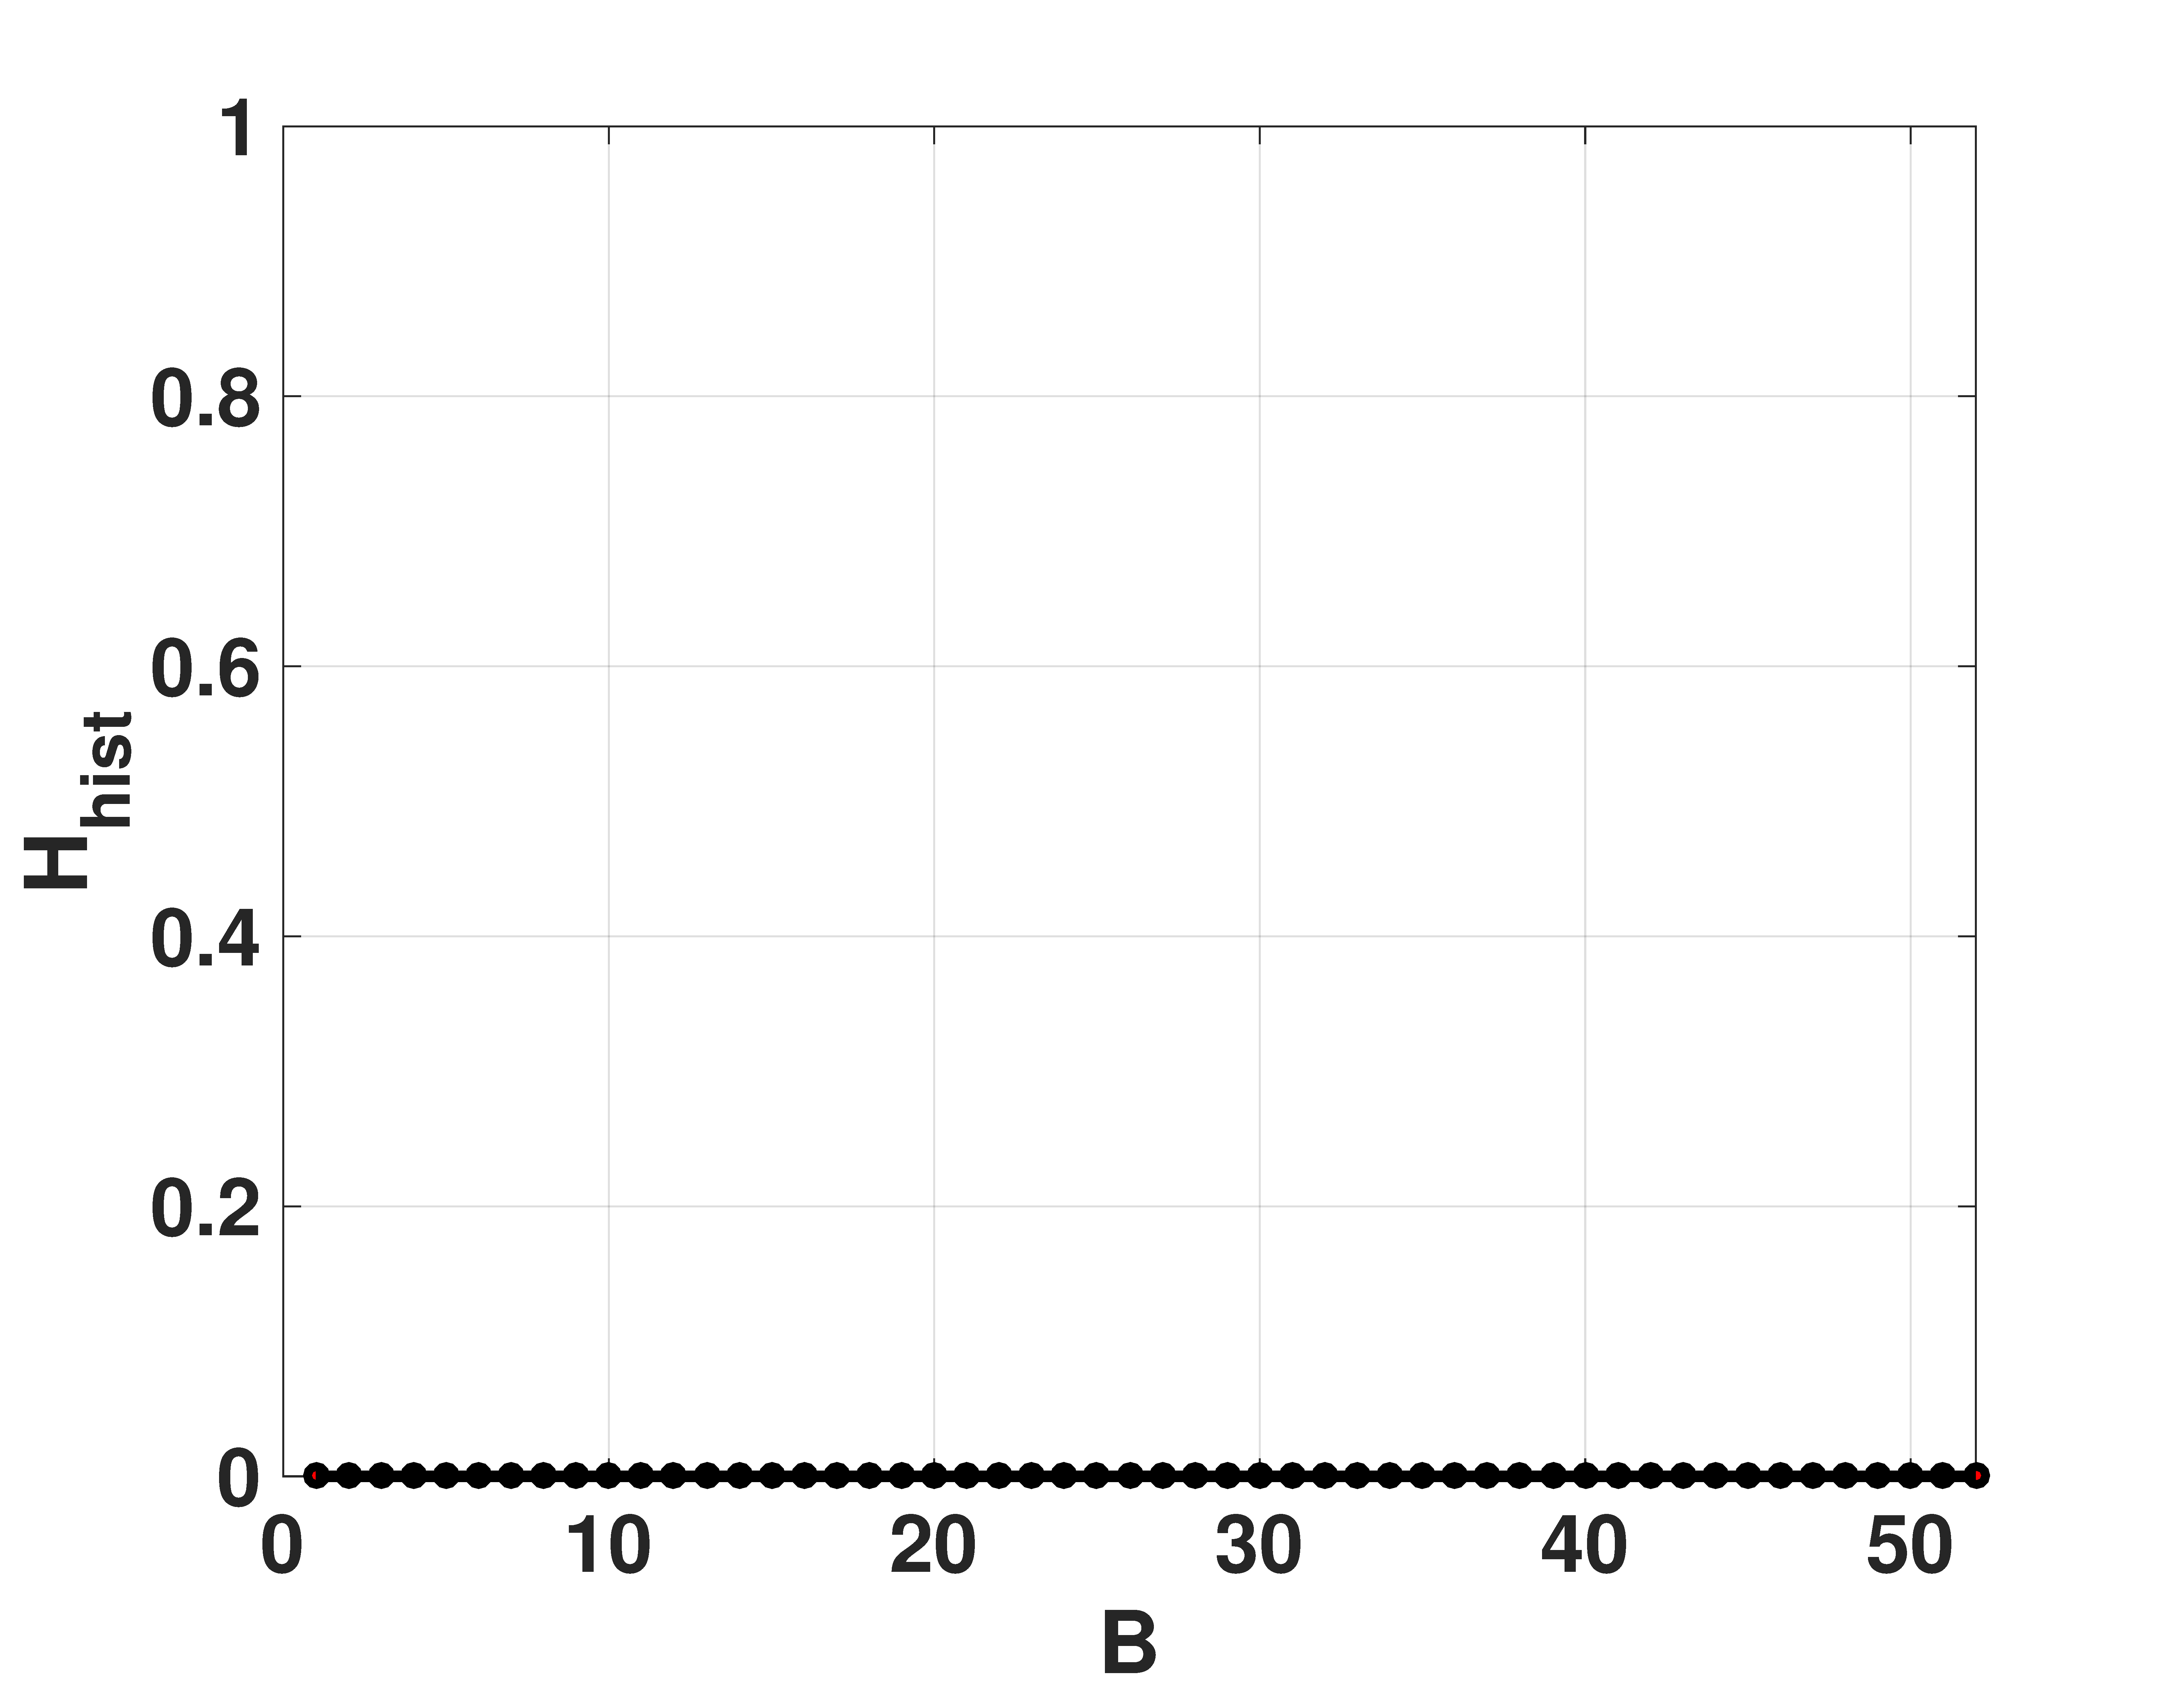
\includegraphics[width=\textwidth]{Hval_Tent}
		\caption{$H_{hist}$ vs. $B$}
		\label{fig:Hval_Tent}
	\end{subfigure}
	\begin{subfigure}[b]{0.49\textwidth}
		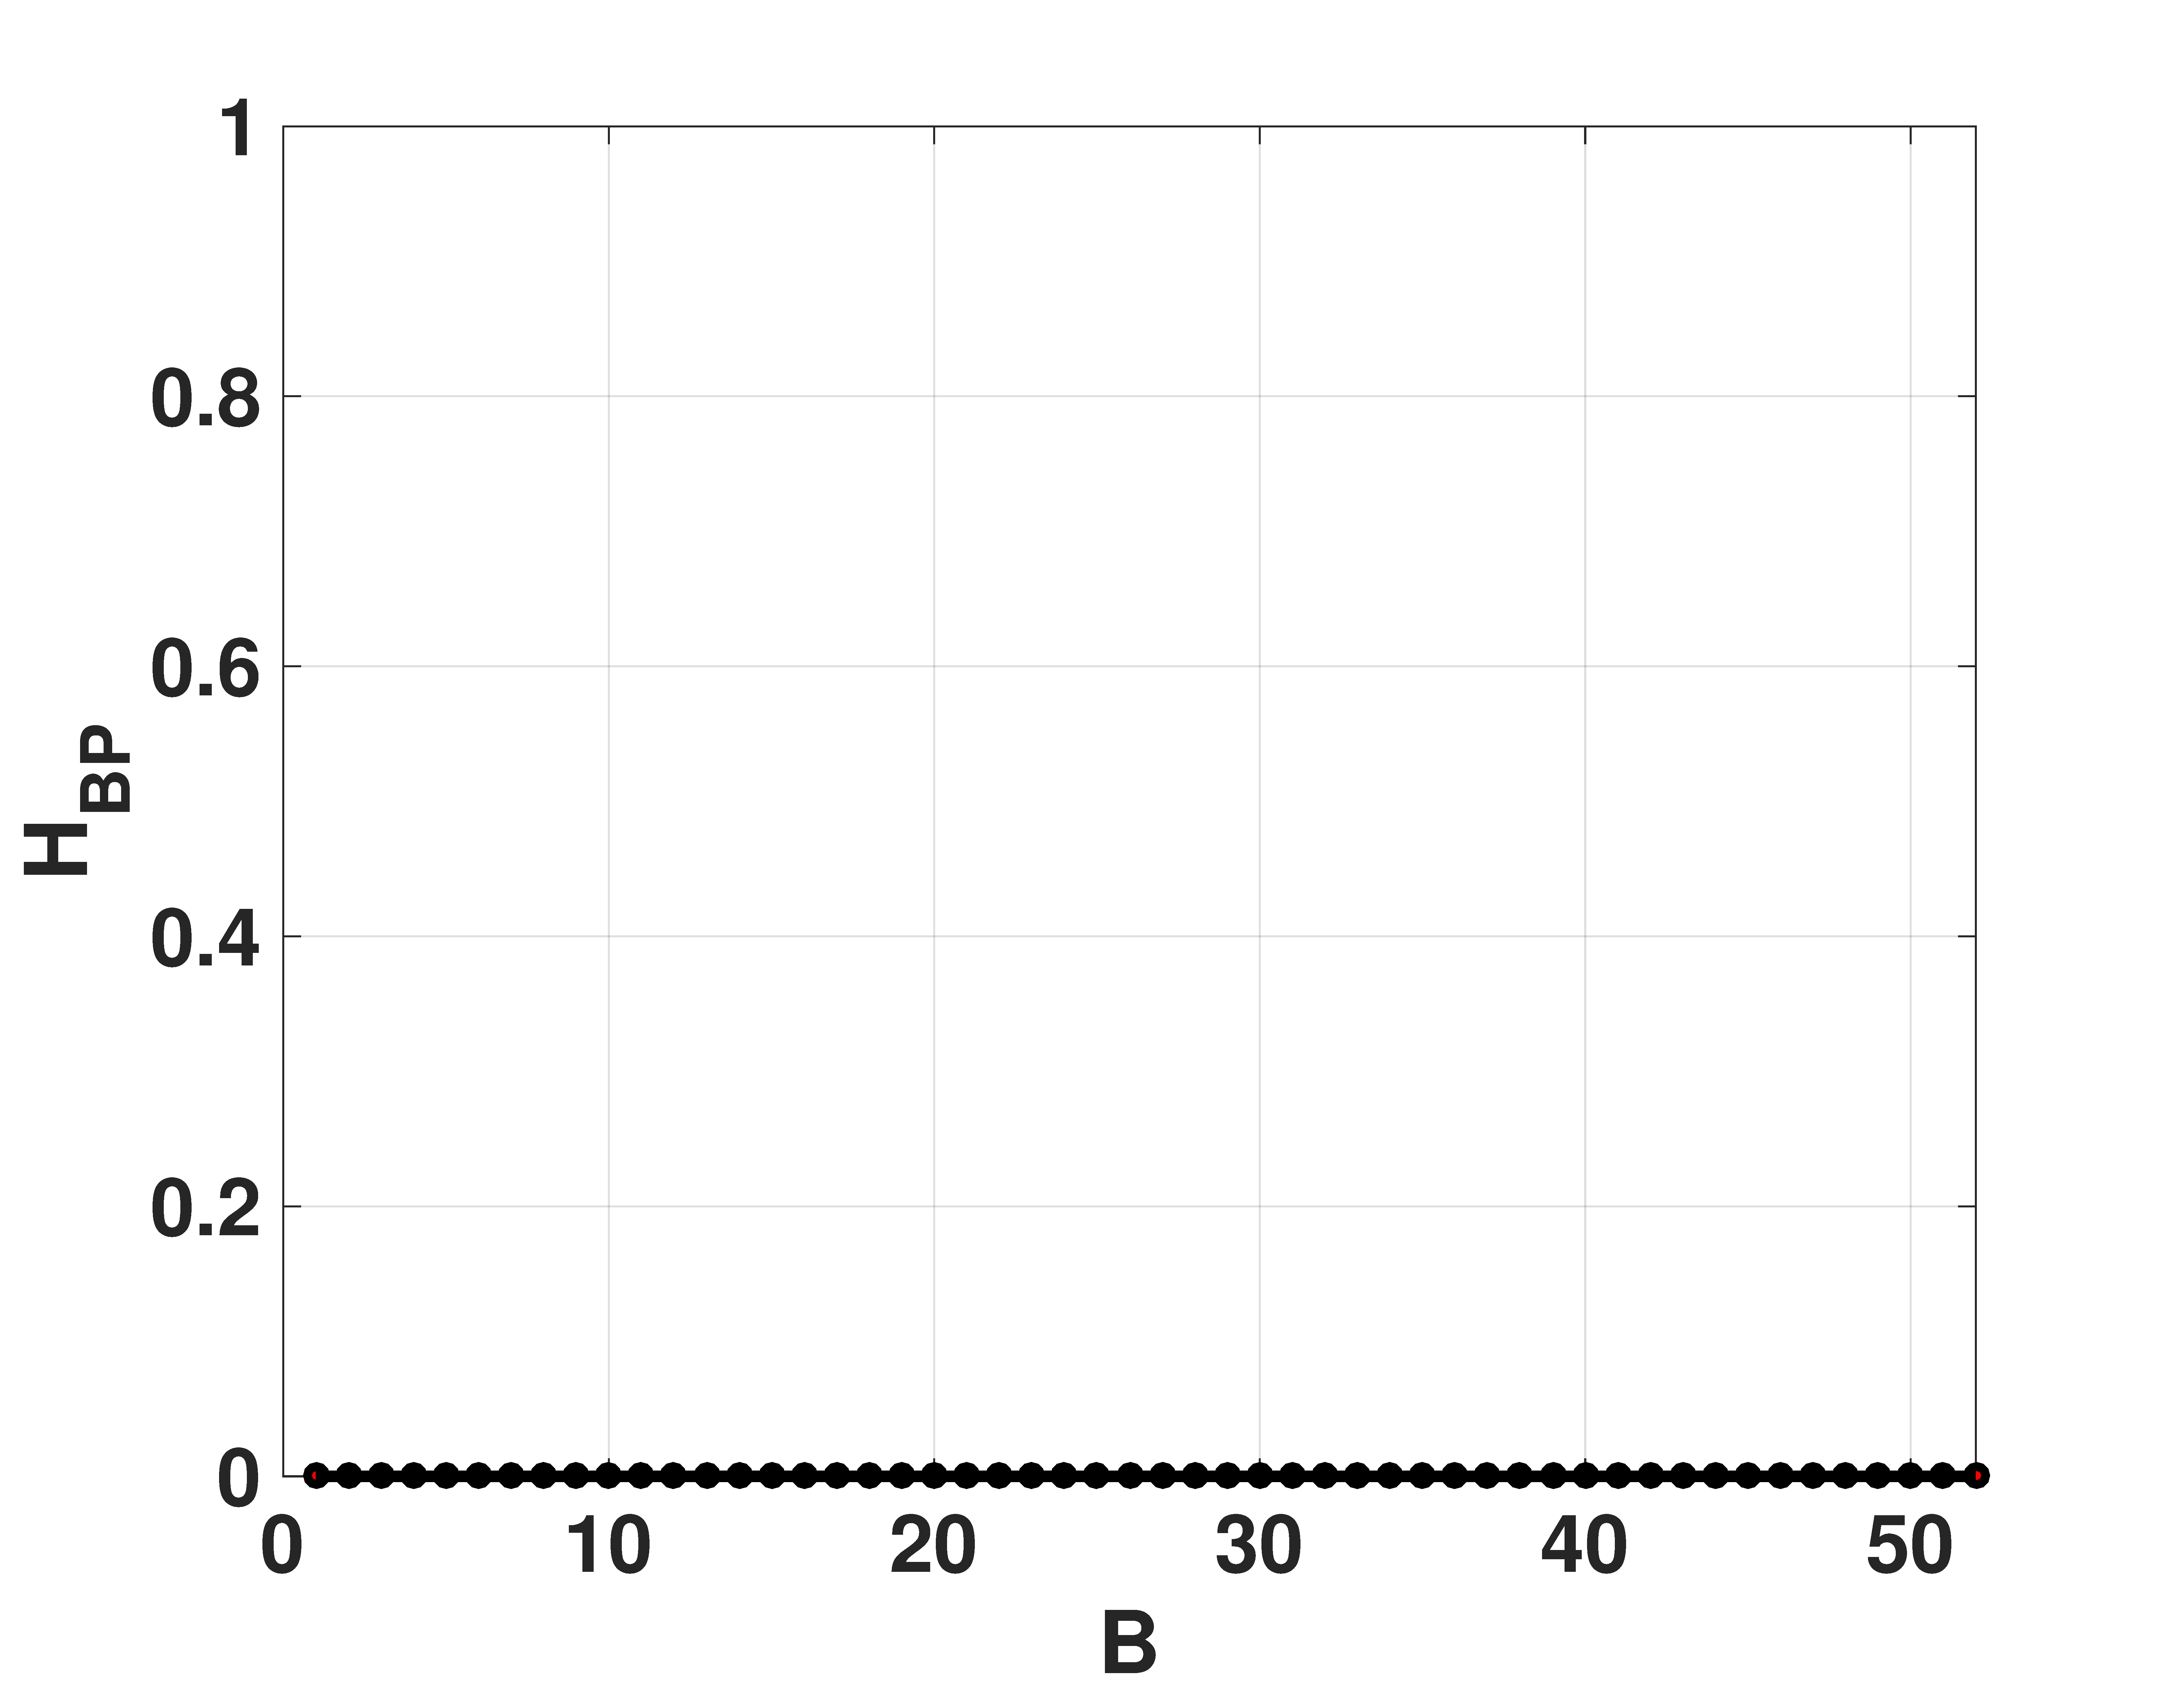
\includegraphics[width=\textwidth]{Hbp_Tent}
		\caption{$H_{BP}$ vs. $B$}
		\label{fig:Hbp_Tent}
	\end{subfigure}
	\begin{subfigure}[b]{0.49\textwidth}
		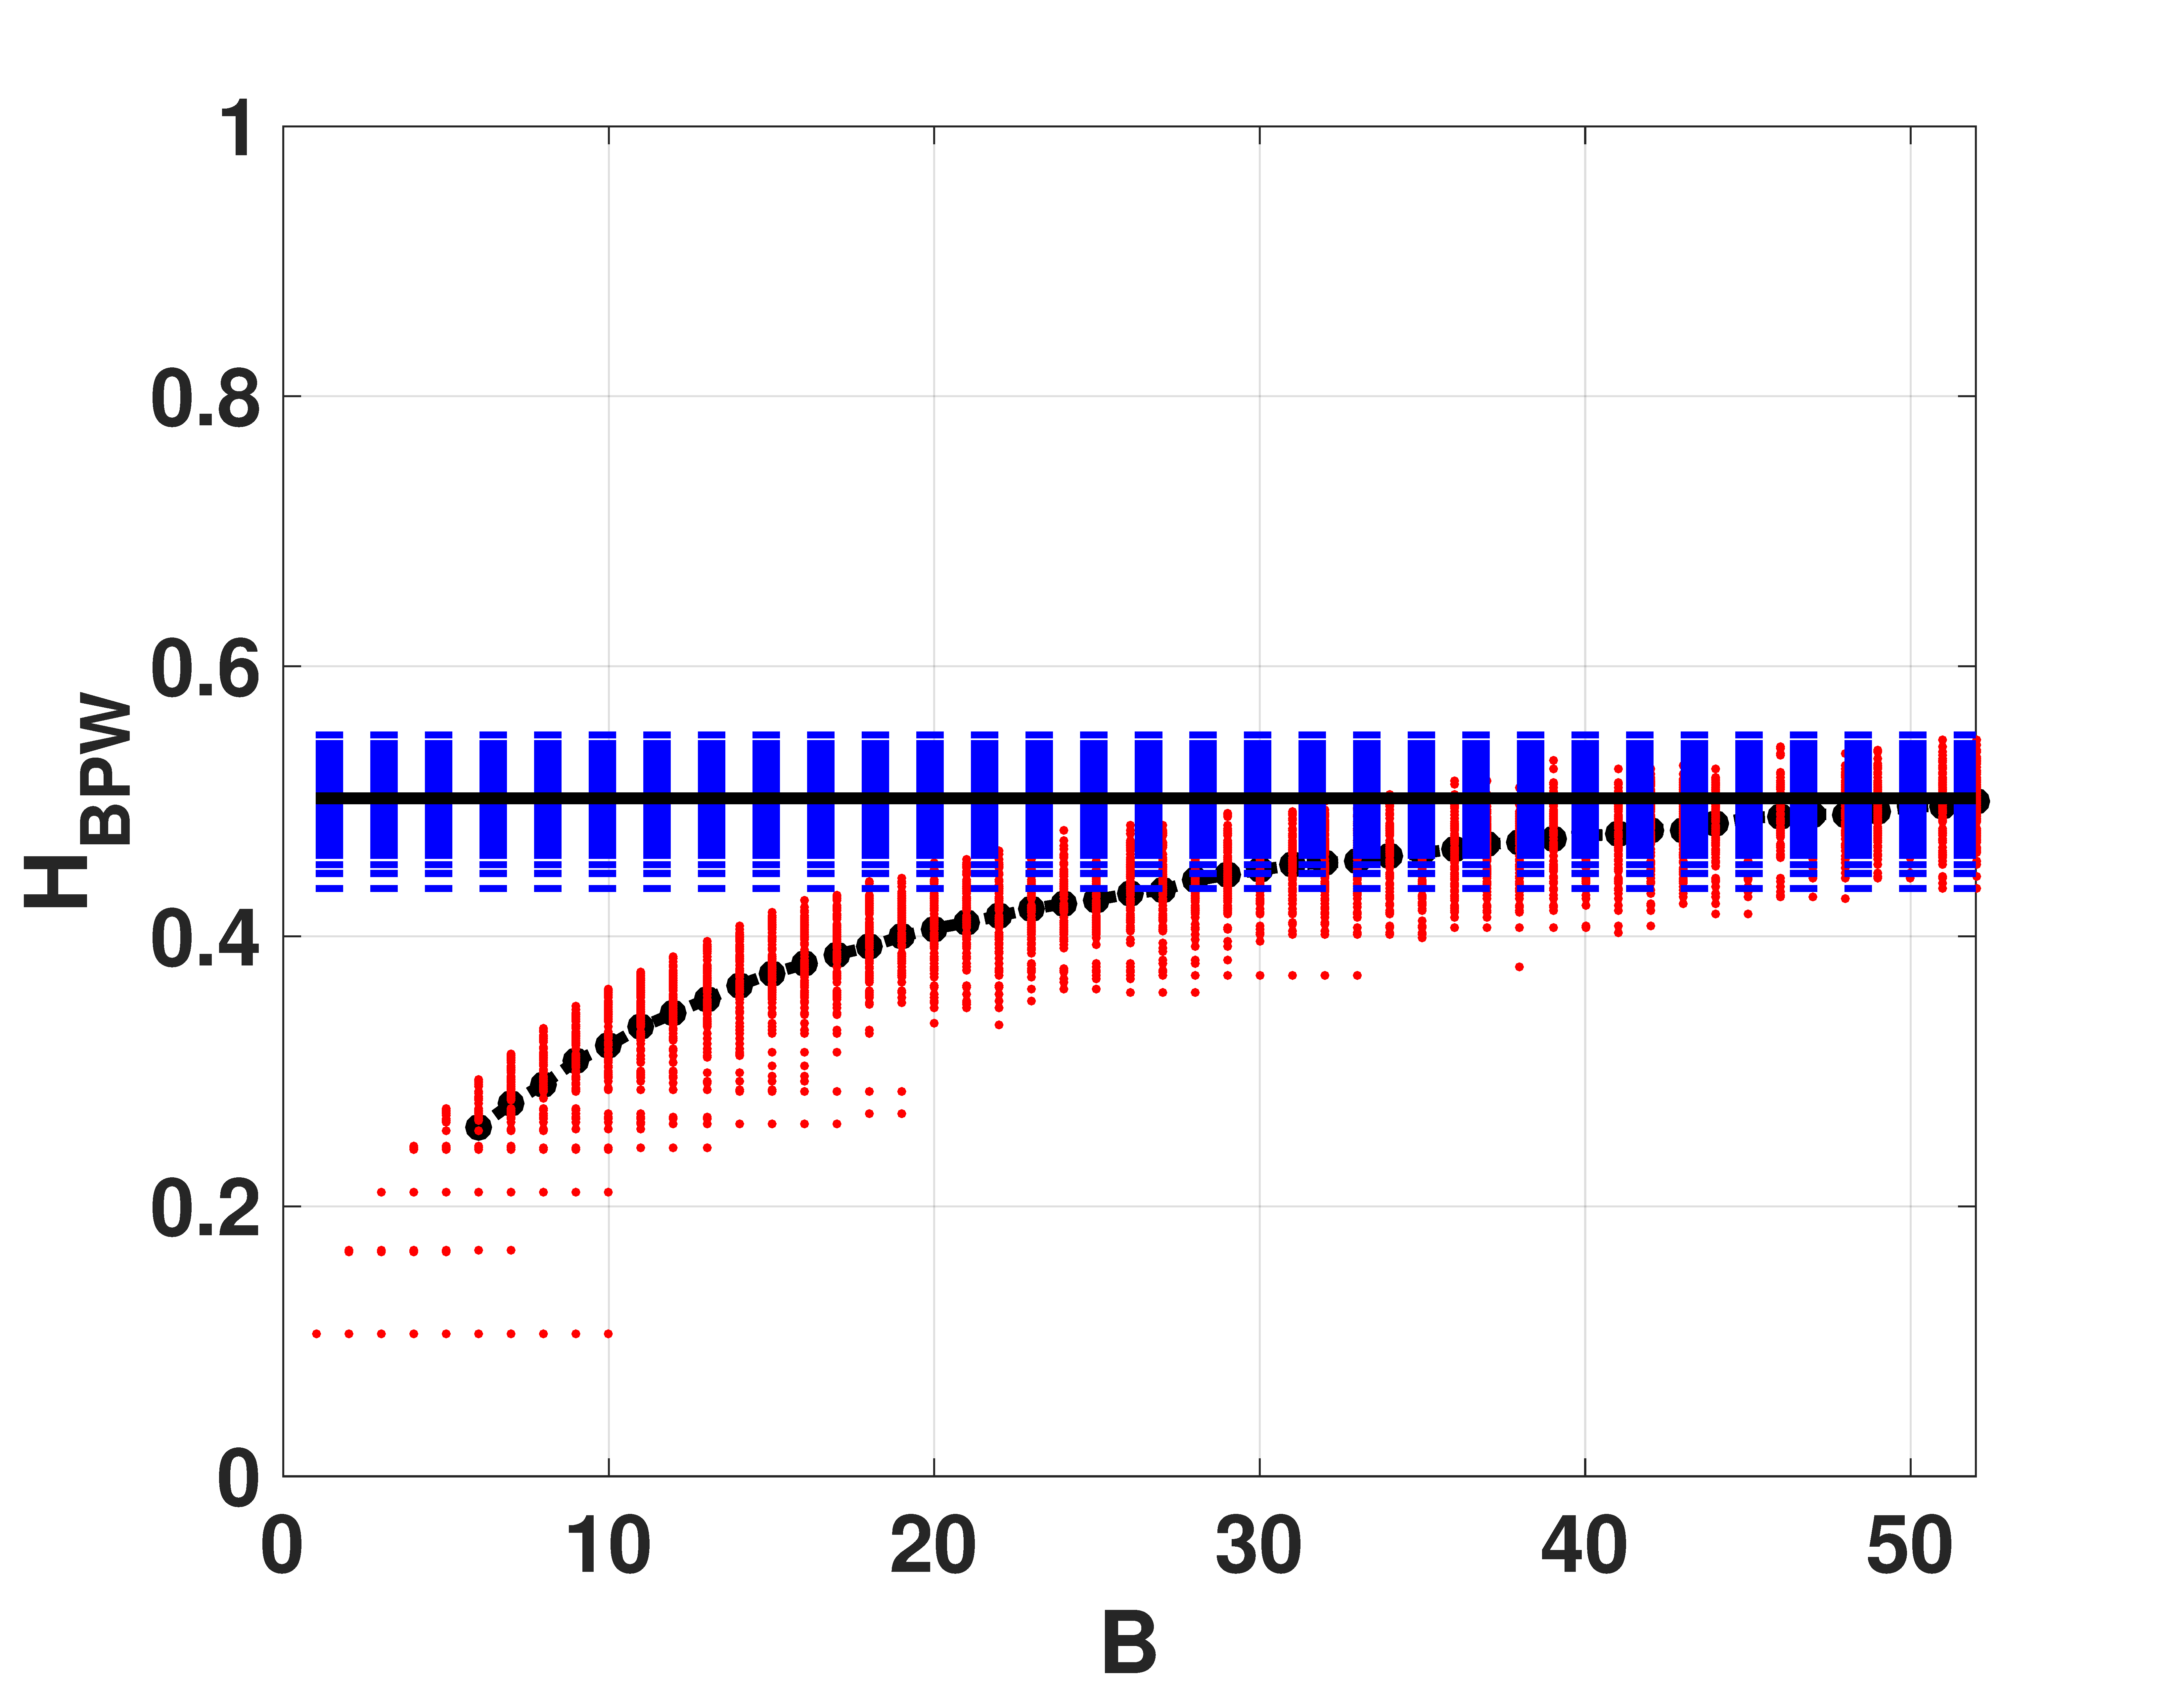
\includegraphics[width=\textwidth]{Hbpw_Tent}
		\caption{$H_{BPW}$ vs. $B$}
		\label{fig:Hbpw_Tent}
	\end{subfigure}
	\begin{subfigure}[b]{0.49\textwidth}
		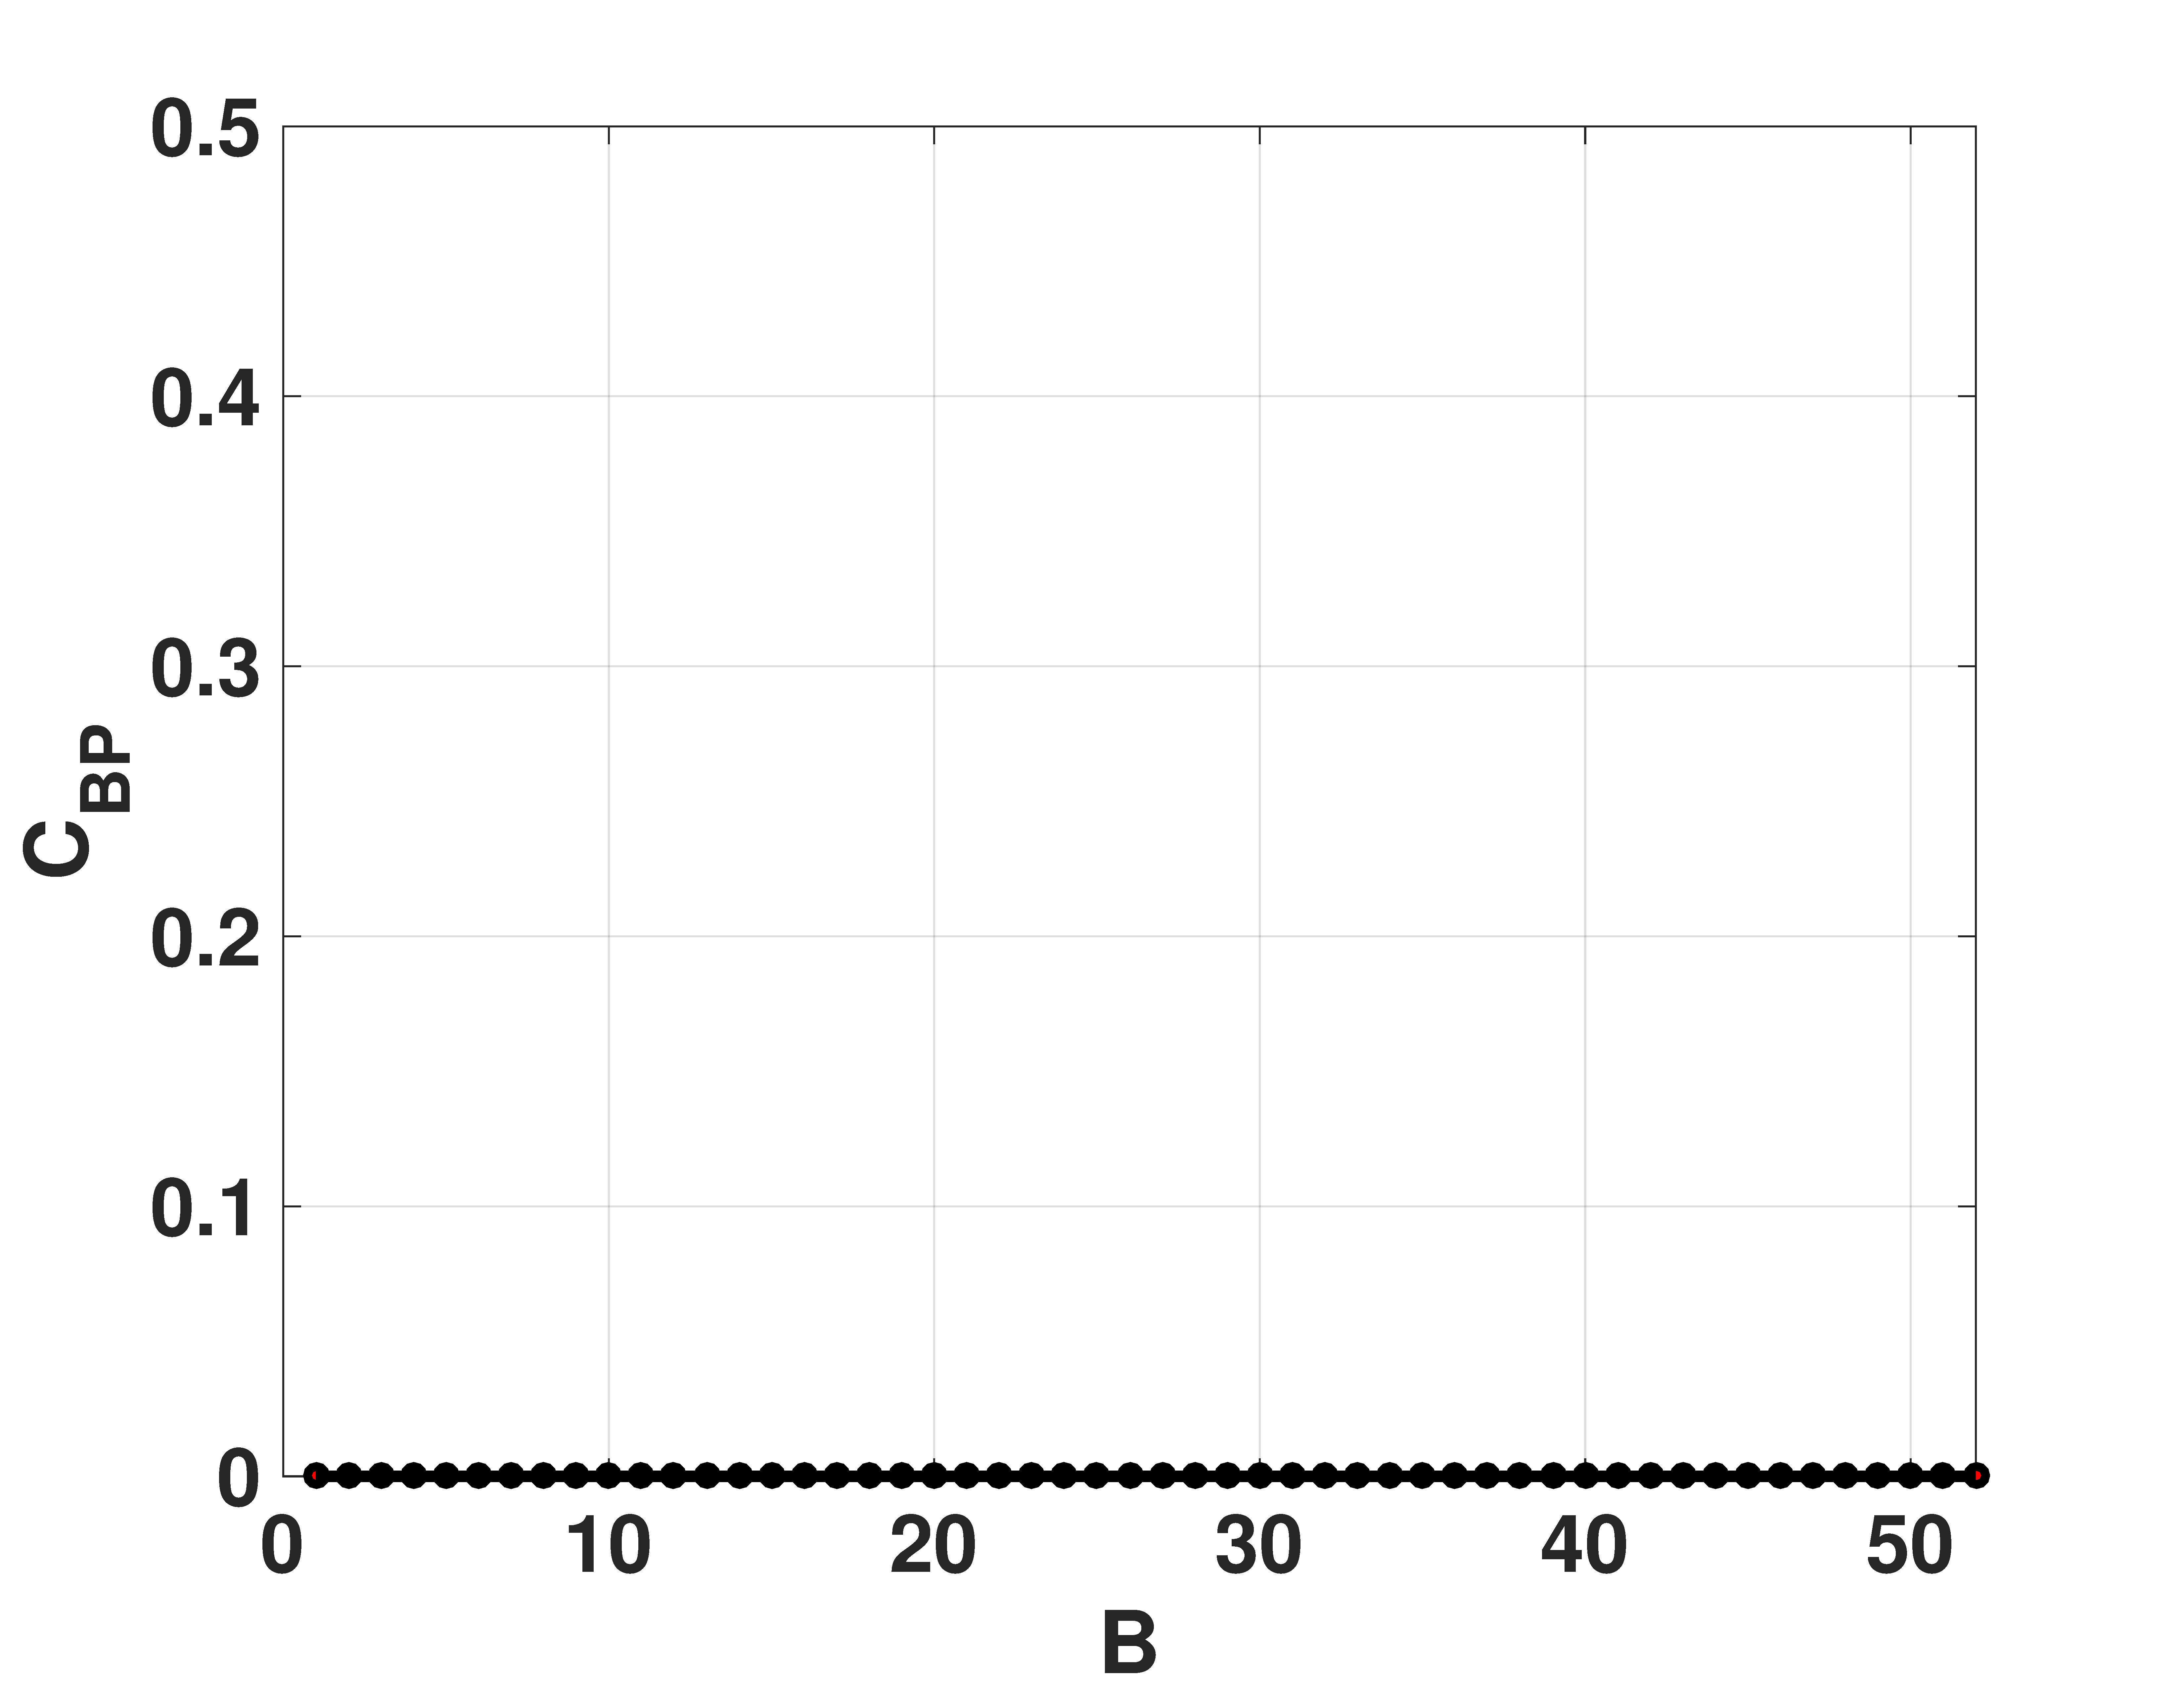
\includegraphics[width=\textwidth]{Cbp_Tent}
		\caption{$C_{BP}$ vs. $B$}
		\label{fig:Cbp_Tent}
	\end{subfigure}
	\begin{subfigure}[b]{0.49\textwidth}
		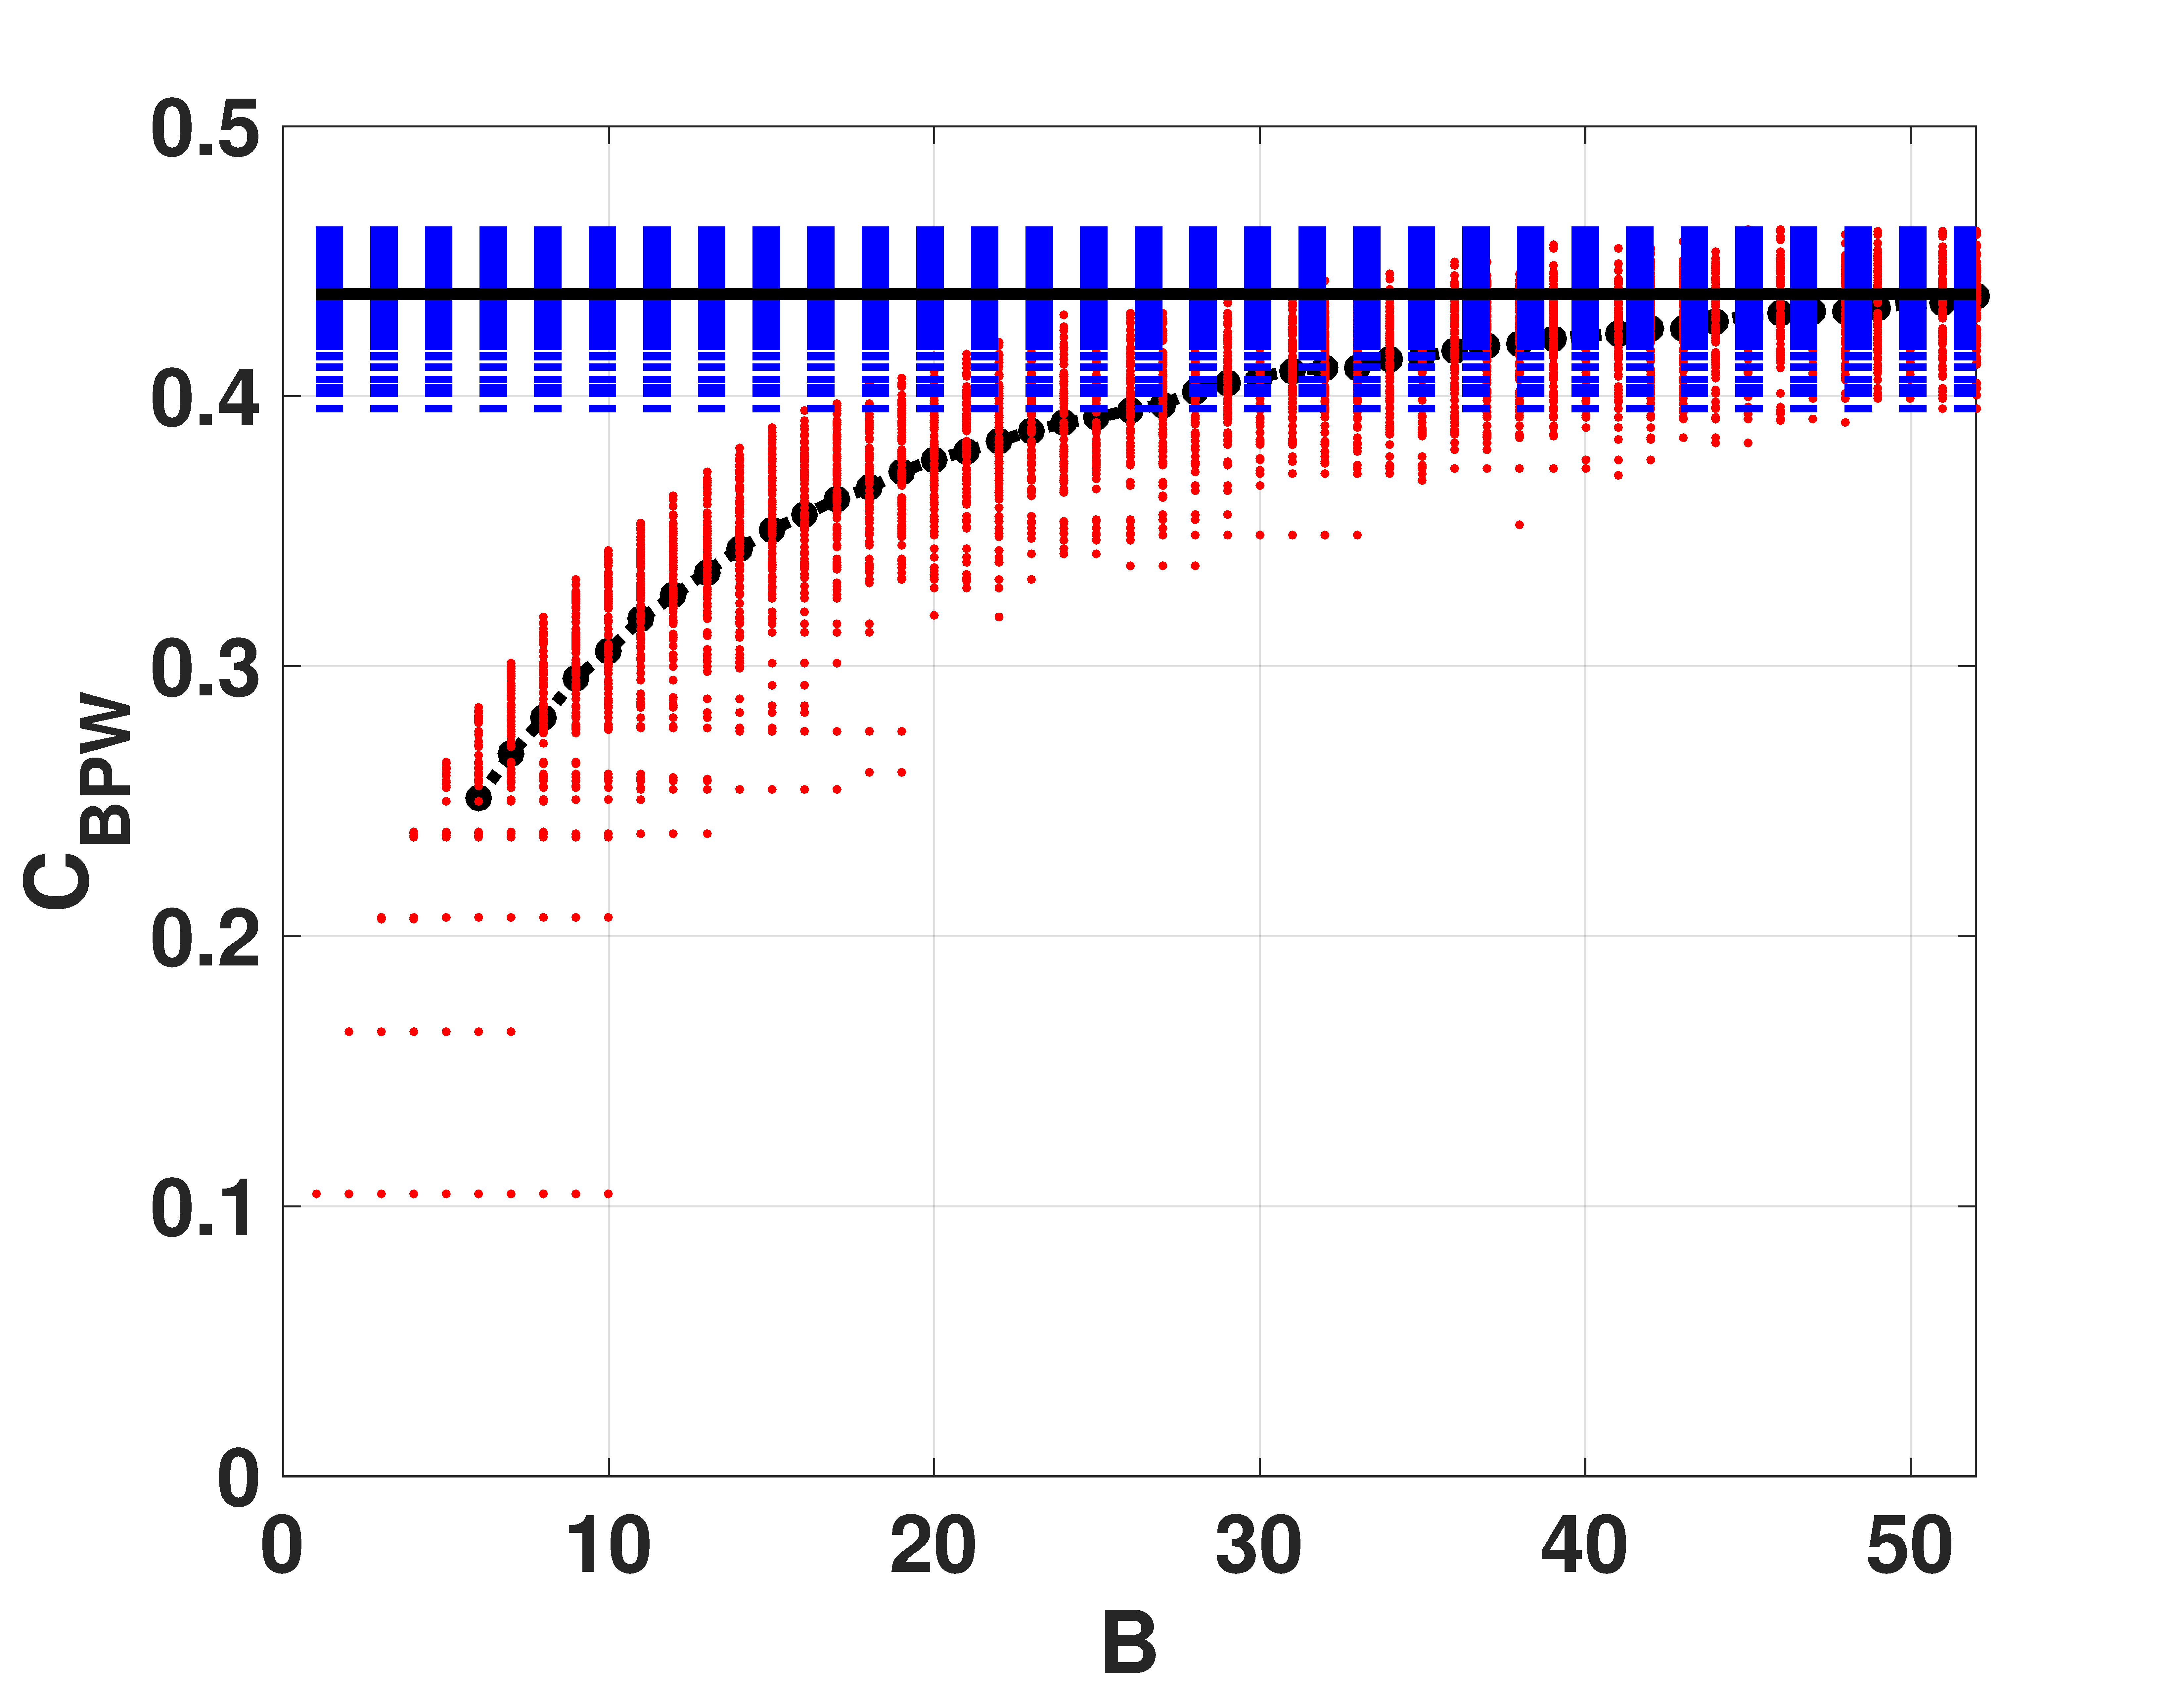
\includegraphics[width=\textwidth]{Cbpw_Tent}
		\caption{$C_{BPW}$ vs. $B$}
		\label{fig:Cbpw_Tent}
	\end{subfigure}
	\begin{subfigure}[b]{0.49\textwidth}
		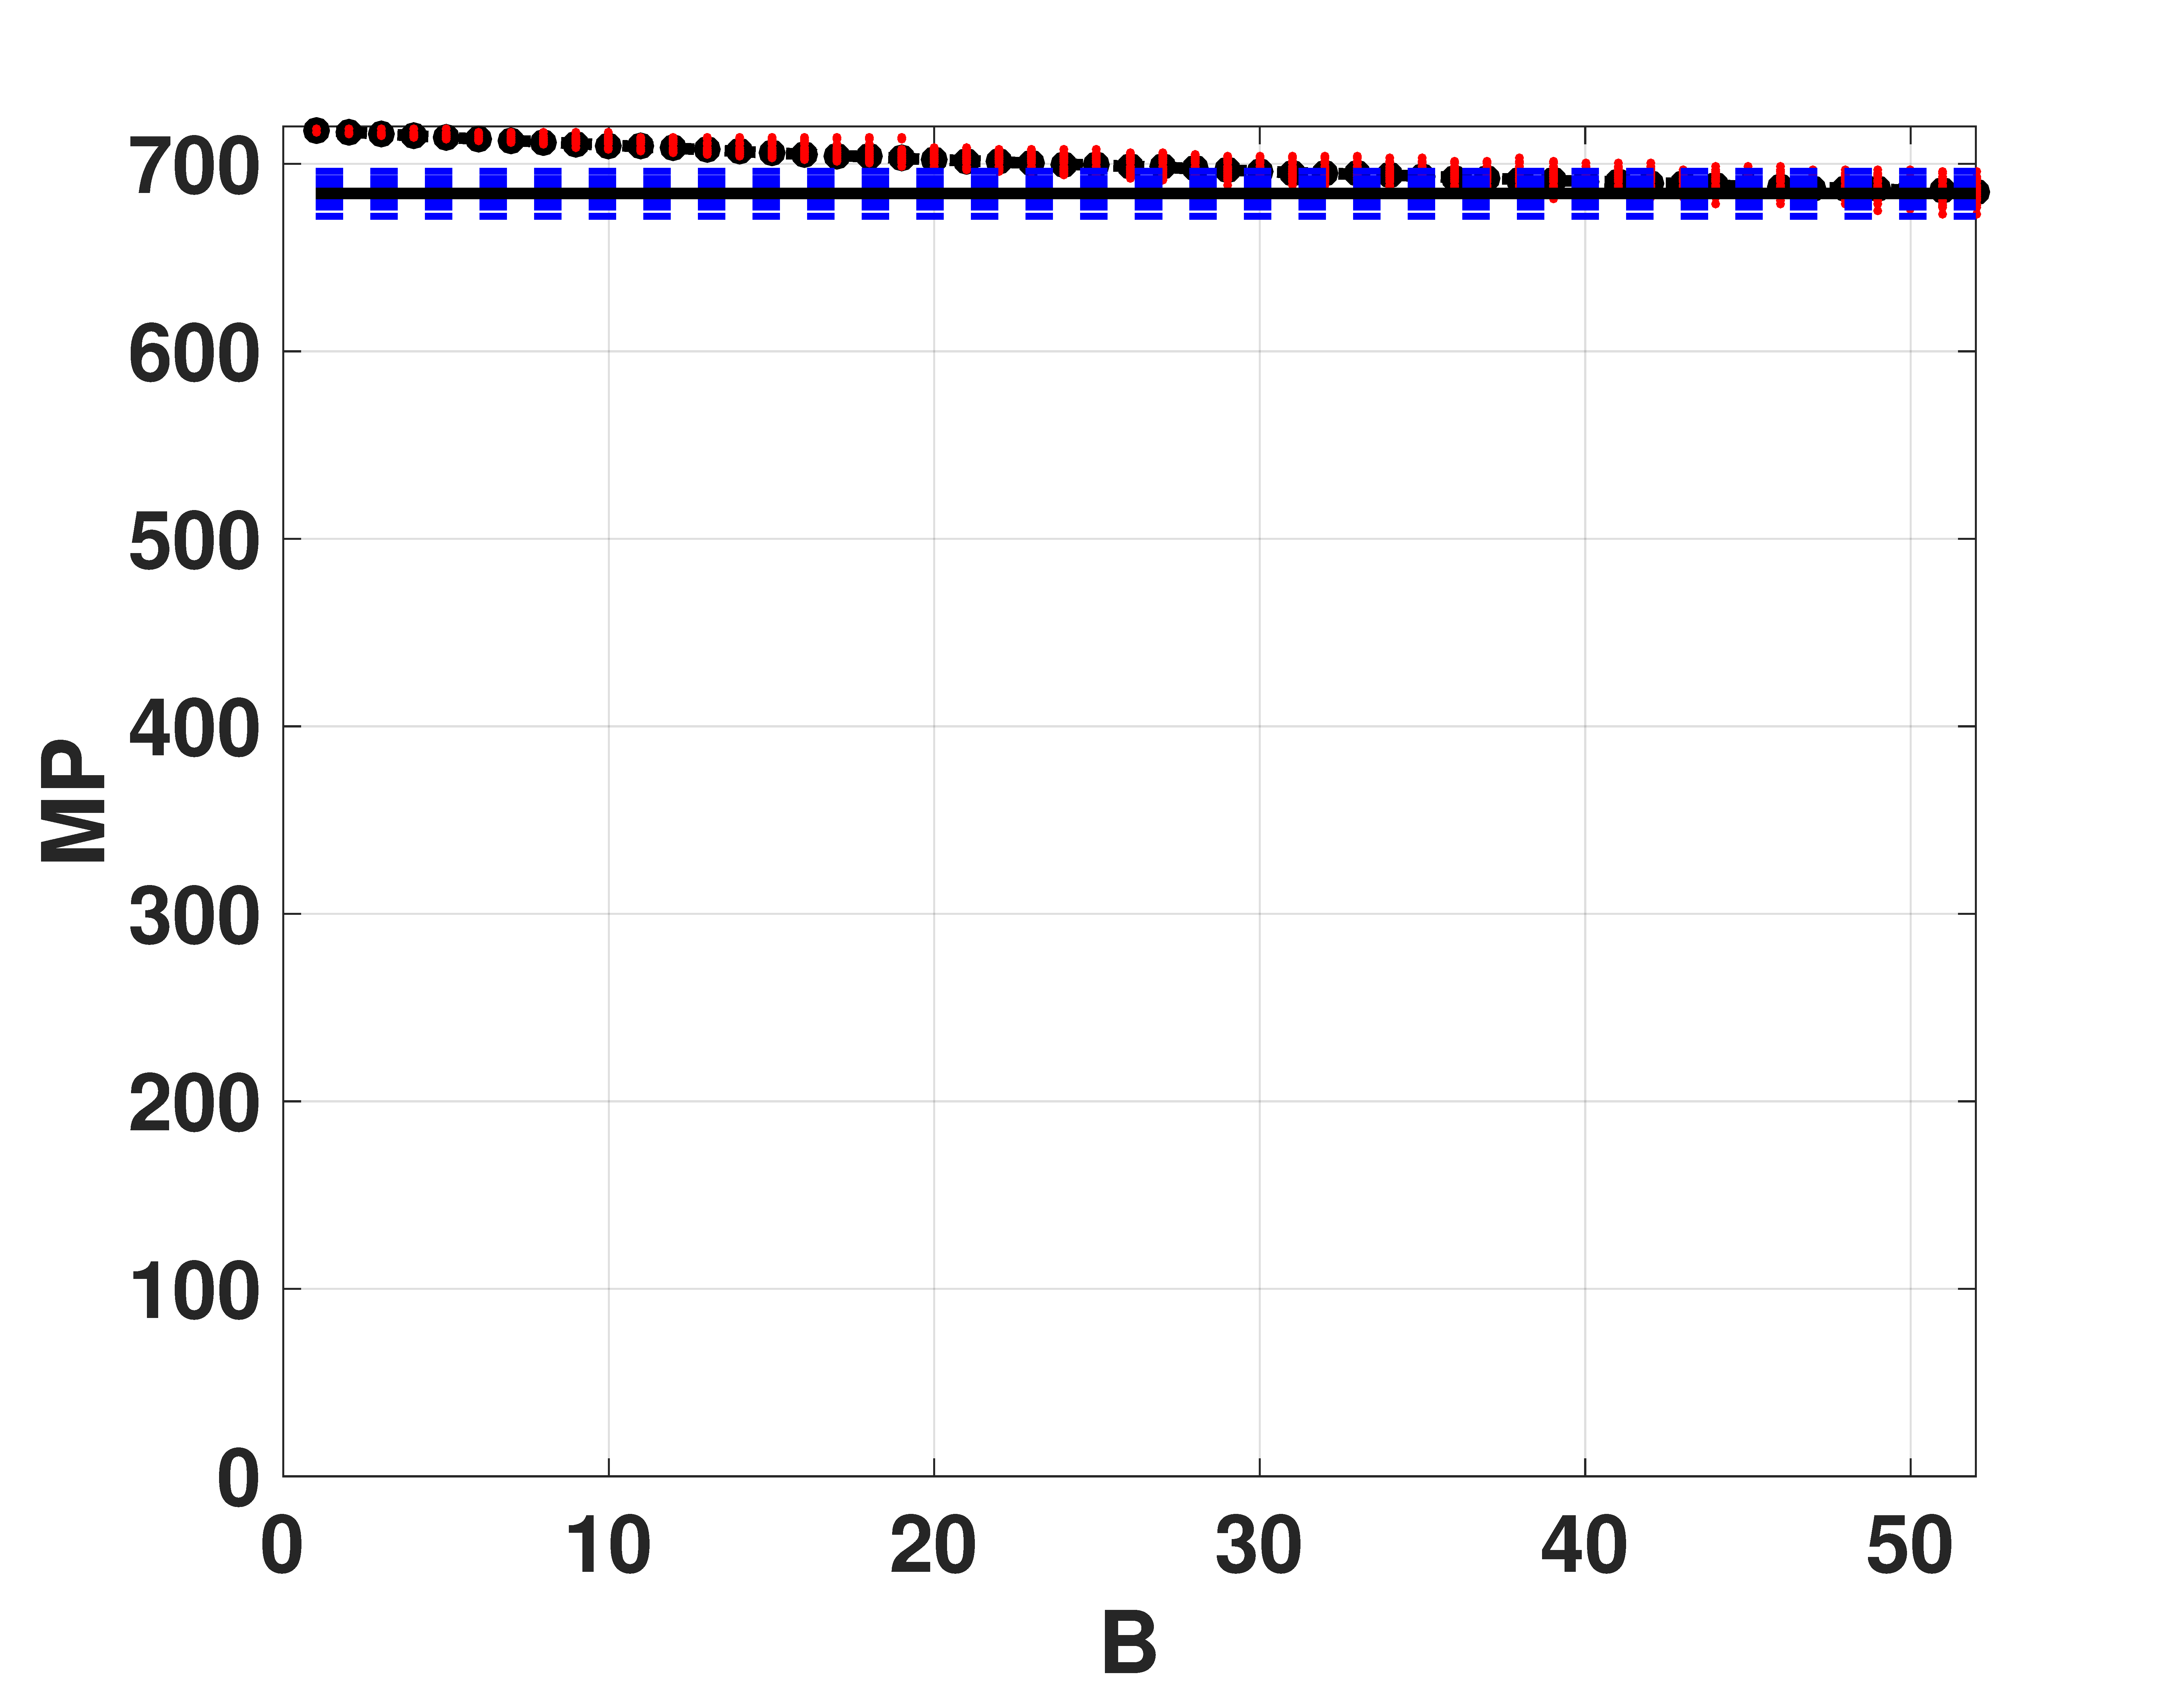
\includegraphics[width=\textwidth]{MP_Tent}
		\caption{MP vs. $B$}
		\label{fig:MP_Tent}
	\end{subfigure}
	\caption{Propiedades estadísticas del mapa TENT con $u=2$.}
	\label{fig:TENT_QuantiB}
\end{figure}
%
Resumiendo, a pesar de usar un alto número de bits (con cualquier representación numérica en base 2) para representar el mapa TENT digitalizado, siempre converge rápidamente al punto fijo en $(x_n, x_{n+1}) = (0, 0)$.

Cuando este mapa se calcula con un valor distinto de $u$ los resultados son completamente distintos, como se muestra en las figuras \ref{fig:TENT1p96_QuantiB}, en donde se muestran los resultados tomando $u=1.96$.
Los resultados son similares a los del mapa LOG, en cuanto a que el valor promediado de los cuantificadores tiendo no monótonamente al valor encontrado en punto flotante y se estabiliza a partir de cierto valor de $B$.
Sin embargo, fueron necesarios más bits de precisión para alcanzar estas asíntotas.
Por otro lado, se puede ver que el valor de $H_{hist}$ es mejor que el encontrado para LOG y que $H_{BP}$ es similar.
Mediante los cuantificadores $H_{BPW}$ y $C_{BPW}$ se puede detectar que con una precisión por debajo de $13$ bits, algunas condiciones iniciales convergen a puntos fijos o divergen, por lo que no es posible utilizar este mapa con $B < 13$.
%
\begin{figure}[htpb]
	\centering
	\begin{subfigure}[b]{0.49\textwidth}
		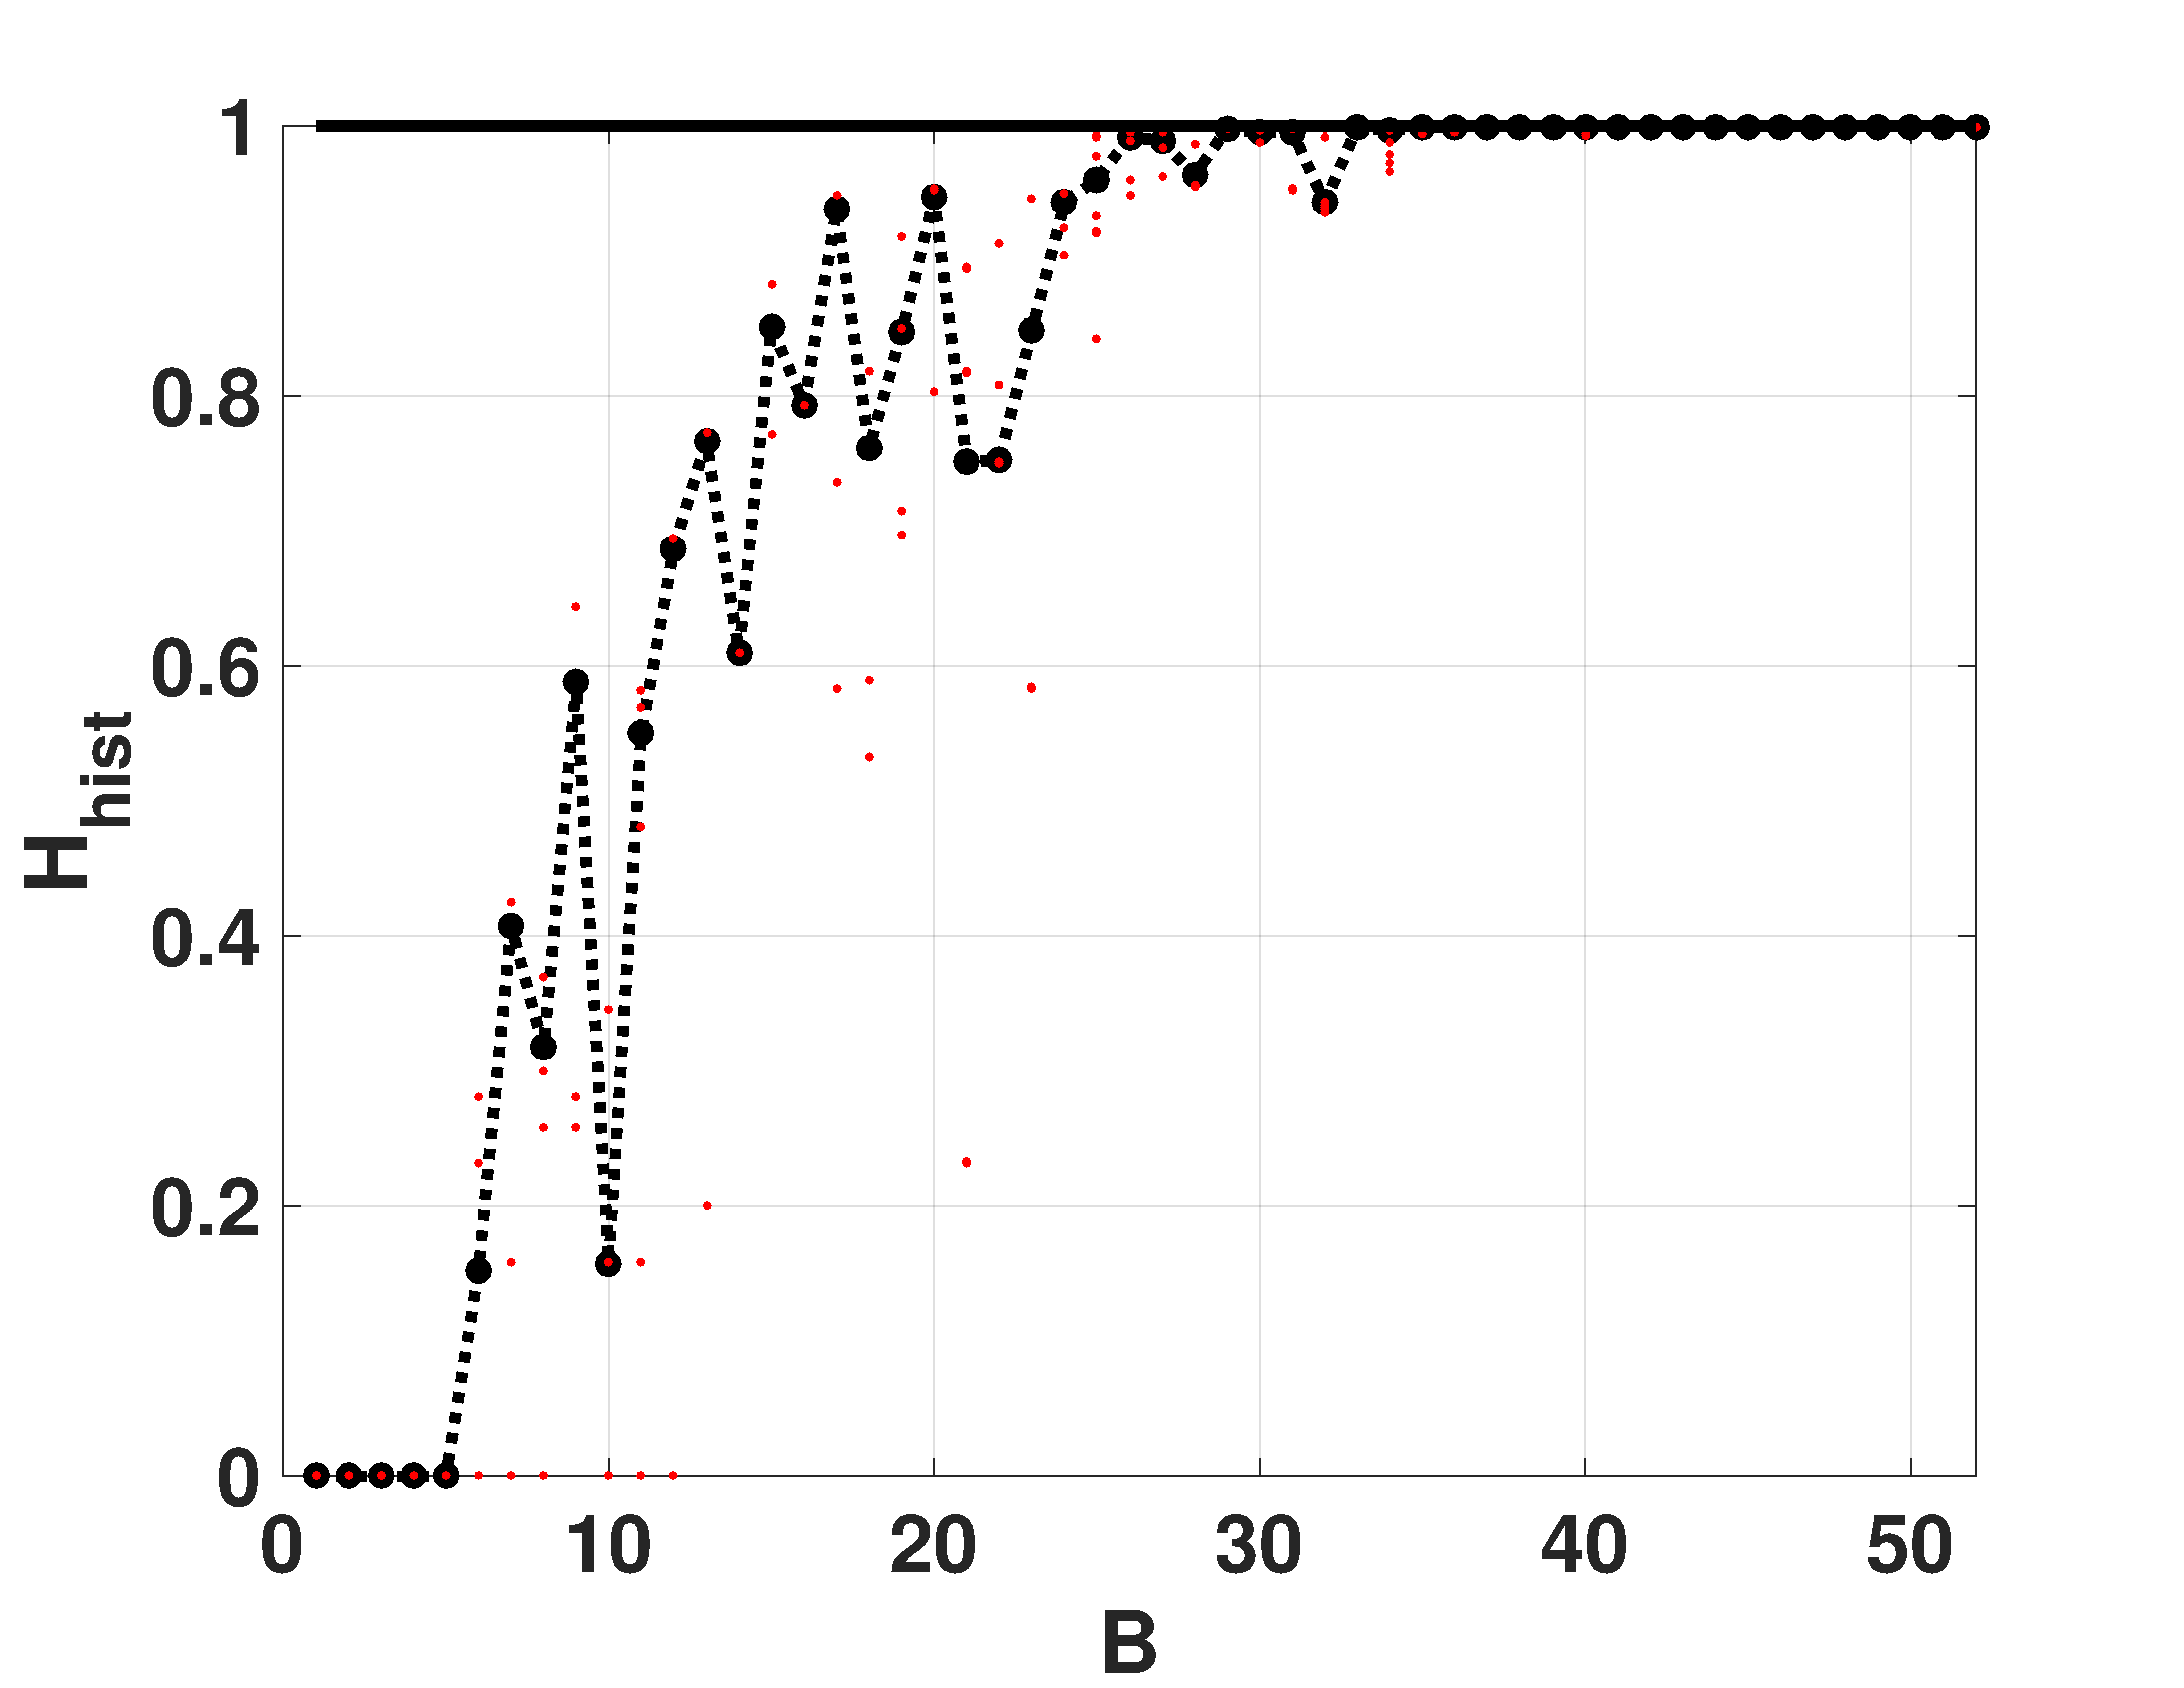
\includegraphics[width=\textwidth]{Hval_Tent1p96}
		\caption{$H_{hist}$ vs. $B$}
		\label{fig:Hval_Tent1p96}
	\end{subfigure}
	\begin{subfigure}[b]{0.49\textwidth}
		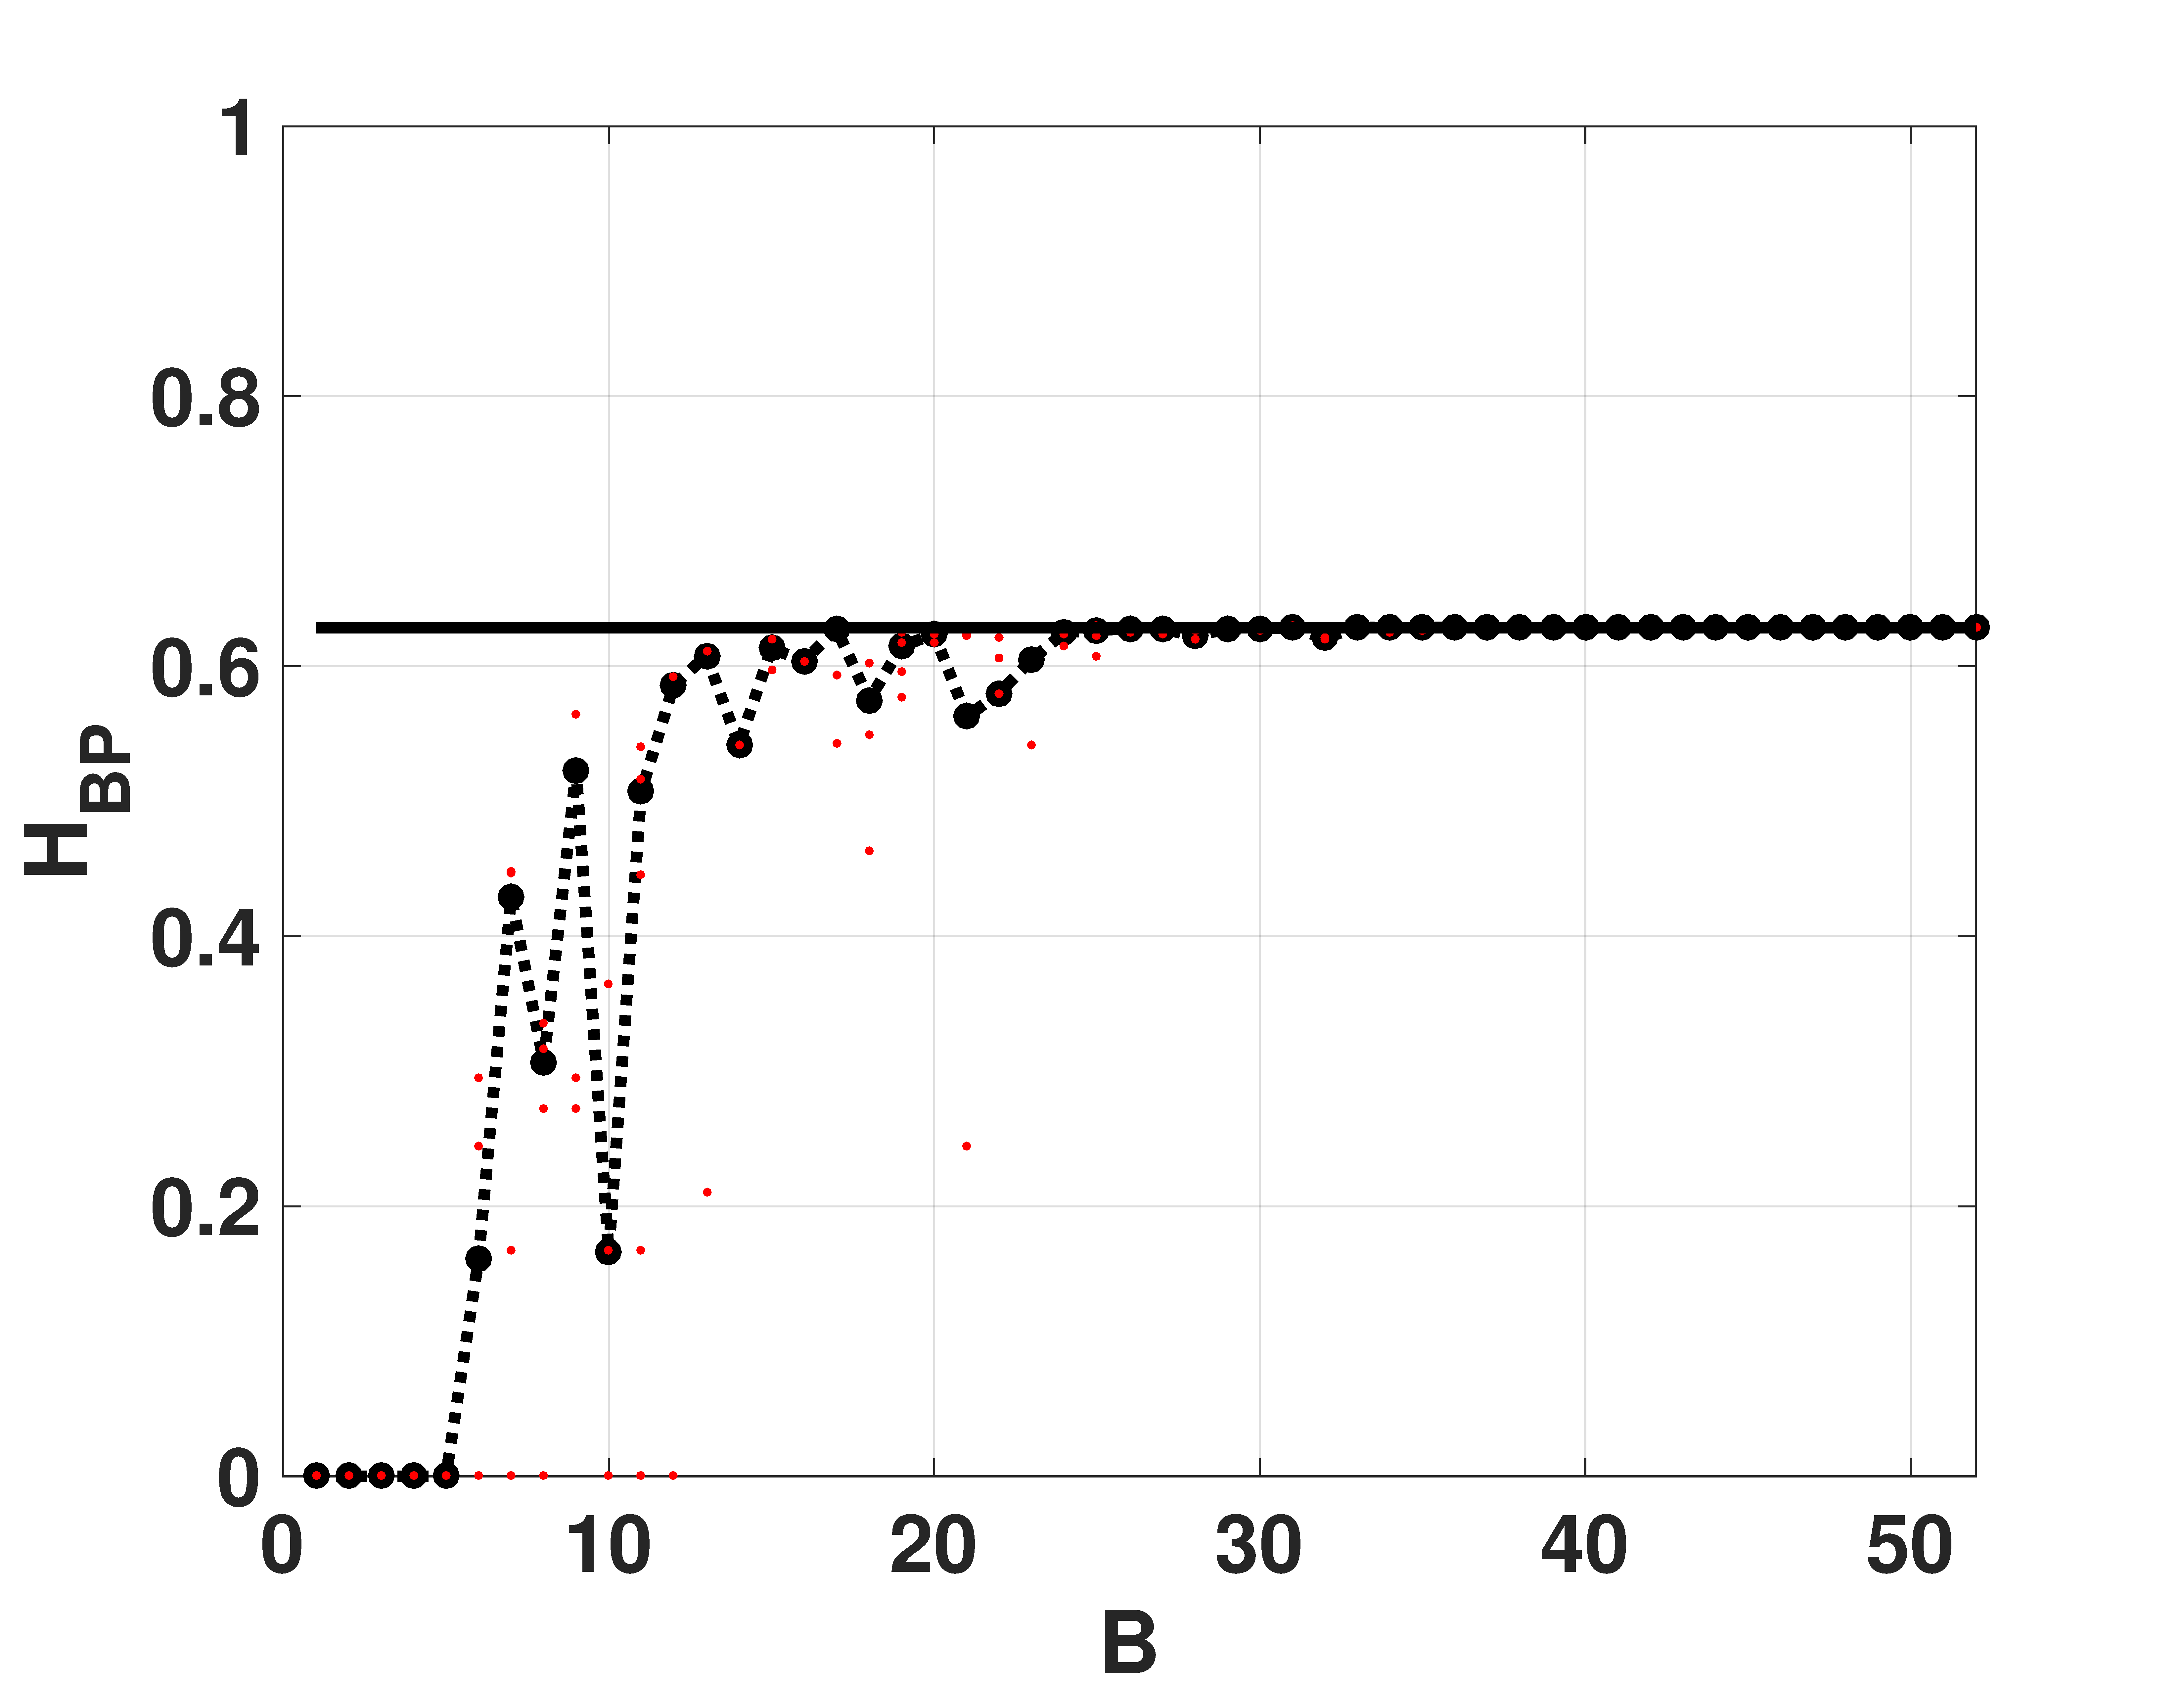
\includegraphics[width=\textwidth]{Hbp_Tent1p96}
		\caption{$H_{BP}$ vs. $B$}
		\label{fig:Hbp_Tent1p96}
	\end{subfigure}
	\begin{subfigure}[b]{0.49\textwidth}
		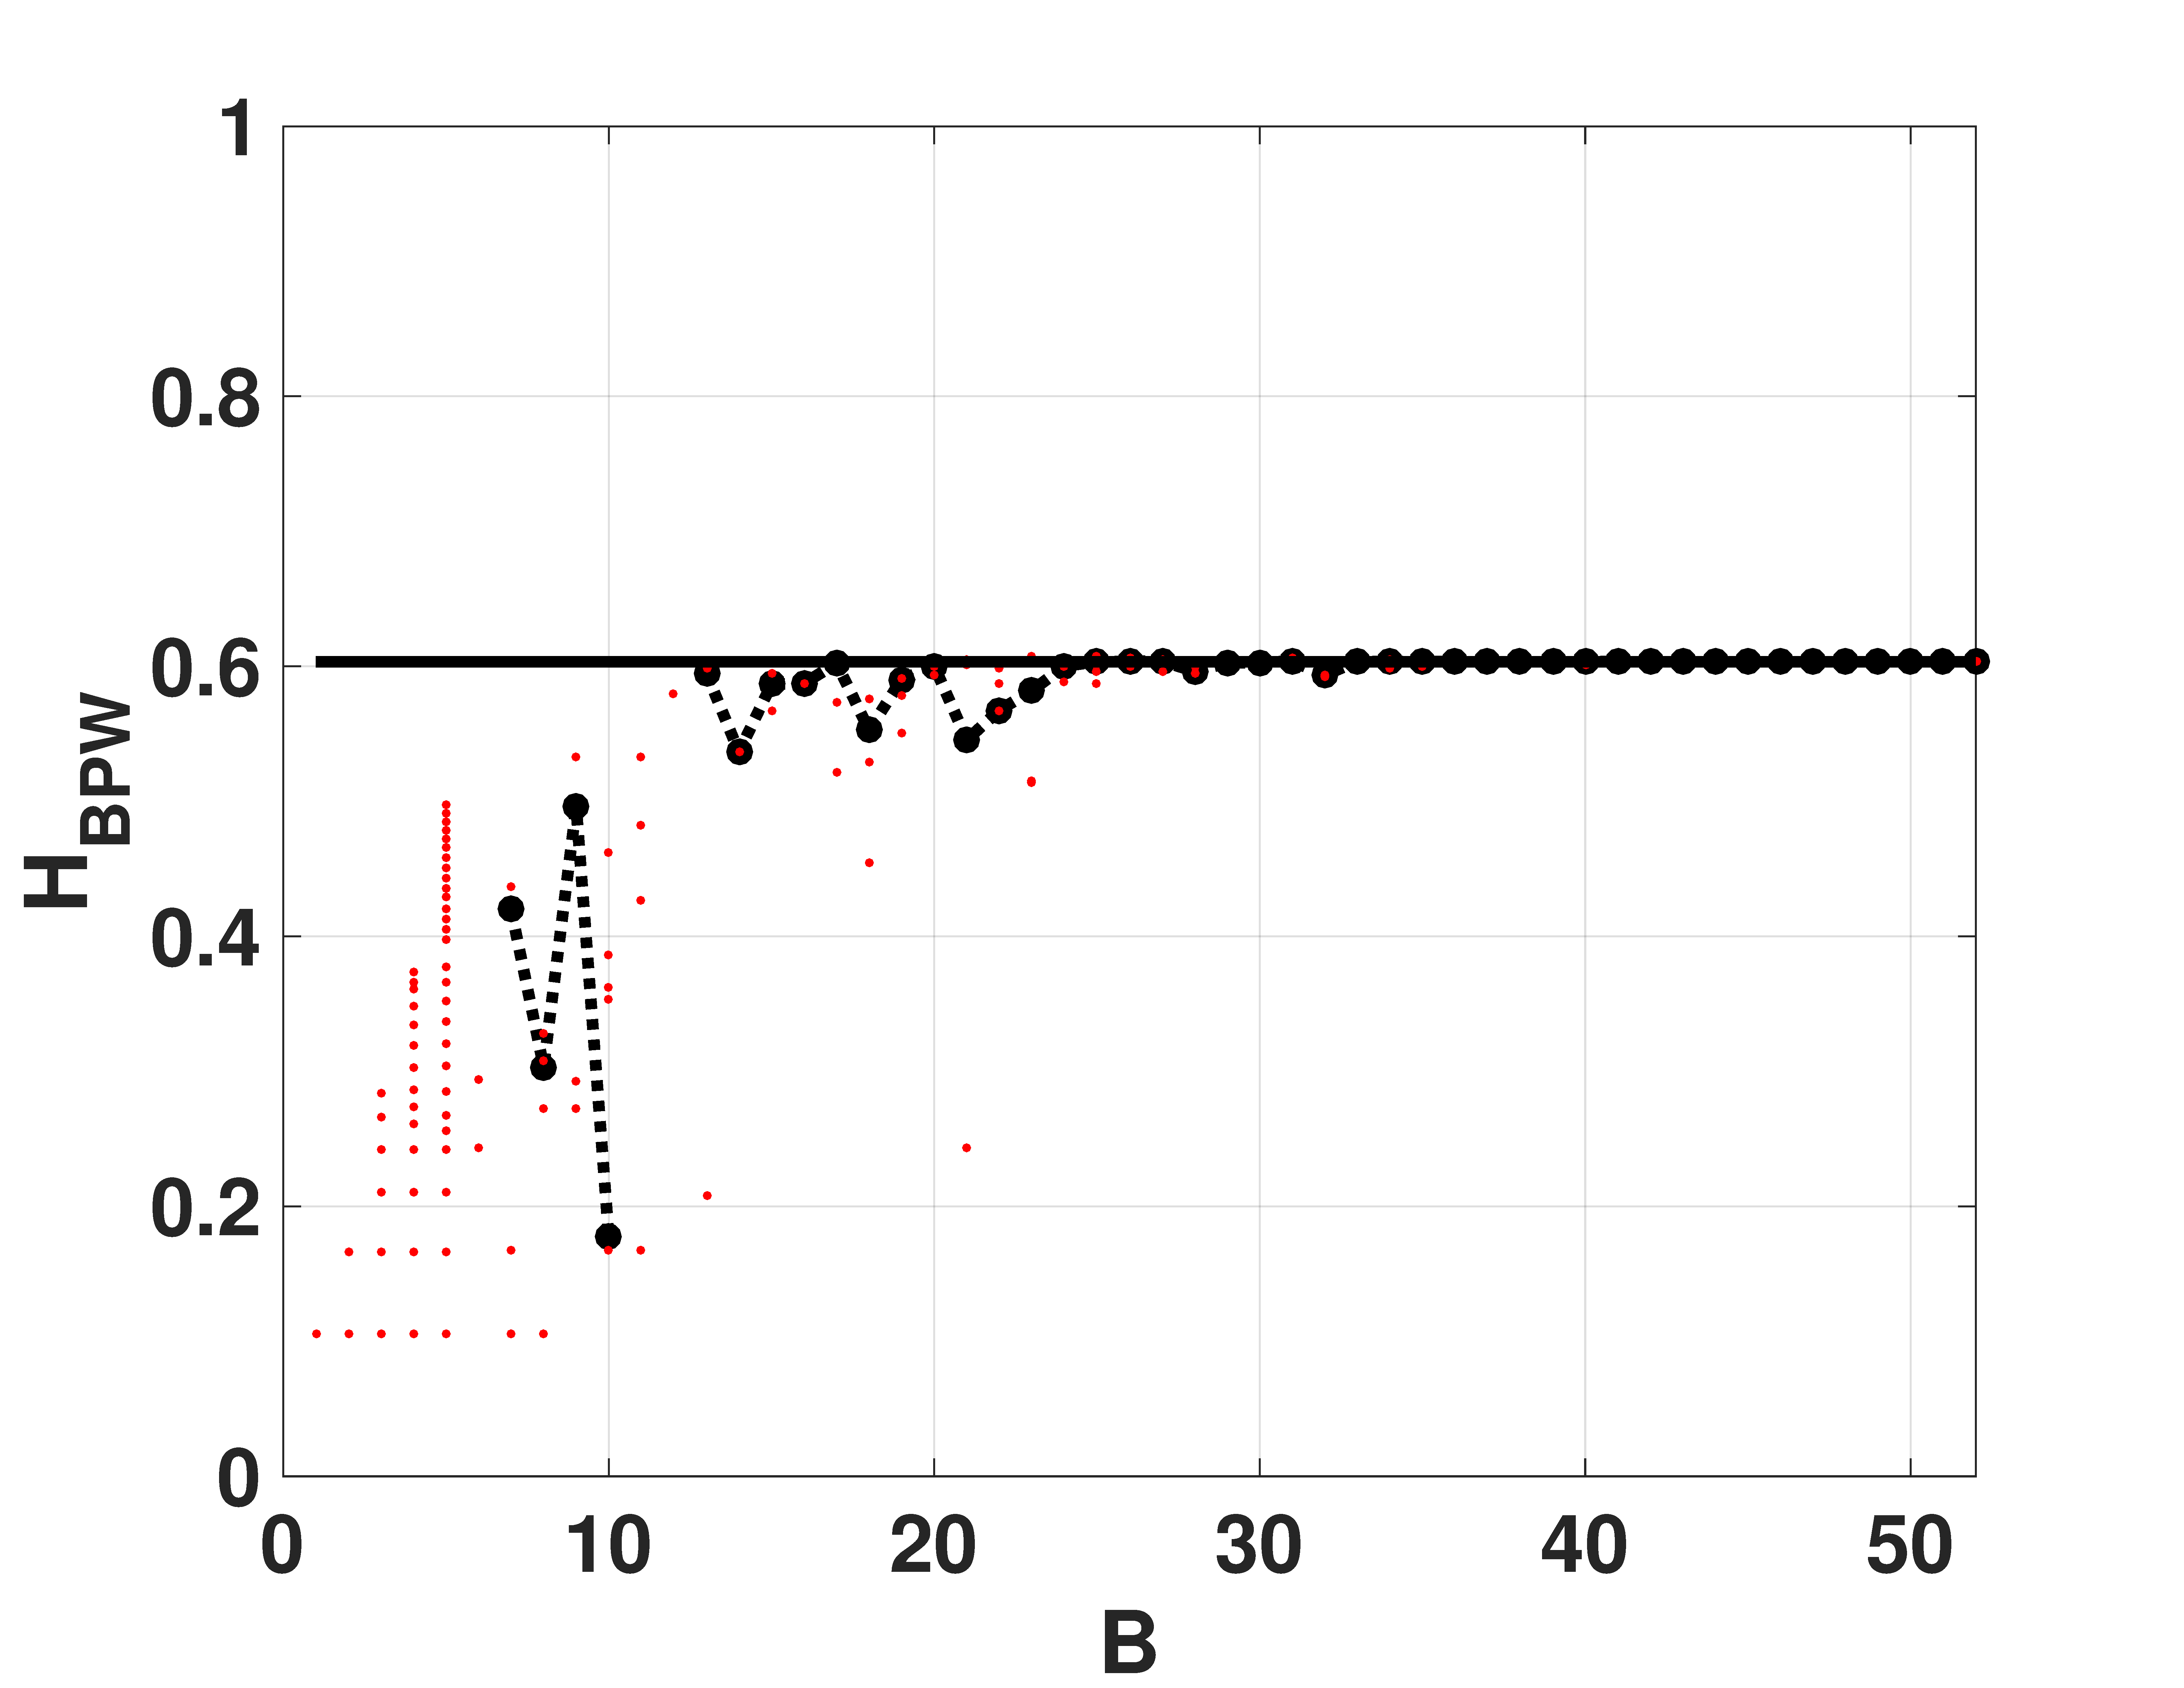
\includegraphics[width=\textwidth]{Hbpw_Tent1p96}
		\caption{$H_{BPW}$ vs. $B$}
		\label{fig:Hbpw_Tent1p96}
	\end{subfigure}
	\begin{subfigure}[b]{0.49\textwidth}
		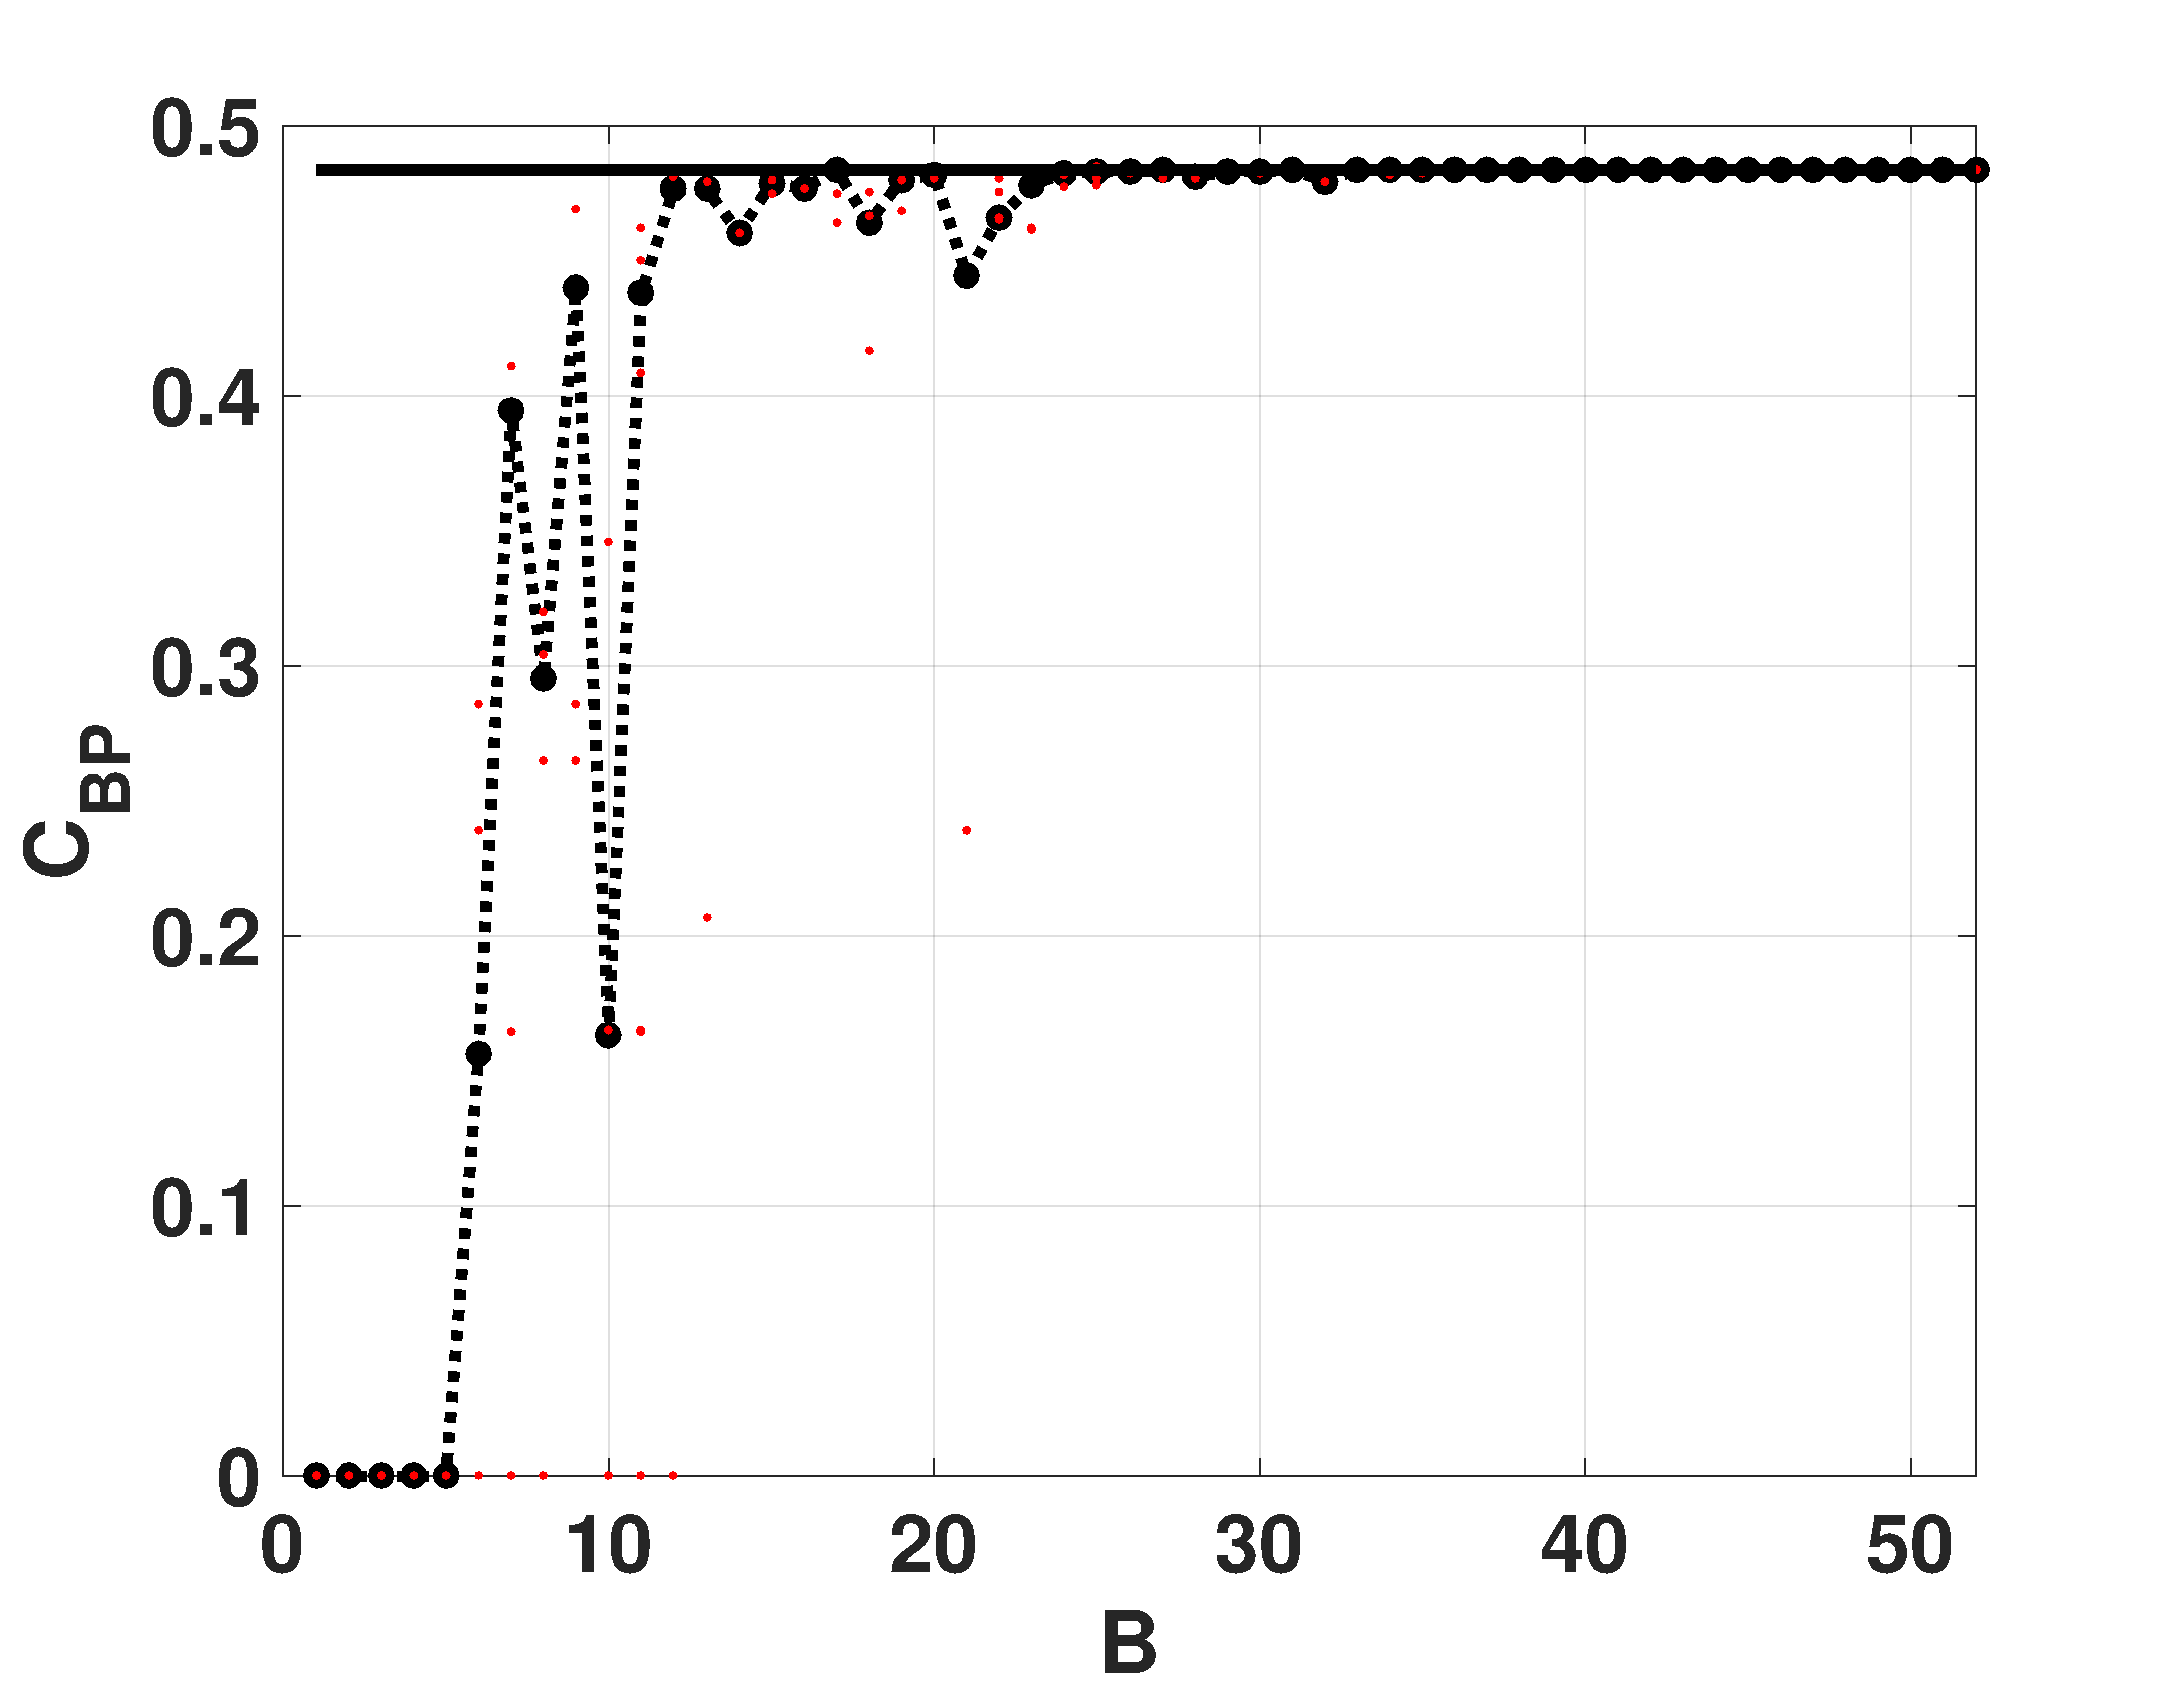
\includegraphics[width=\textwidth]{Cbp_Tent1p96}
		\caption{$C_{BP}$ vs. $B$}
		\label{fig:Cbp_Tent1p96}
	\end{subfigure}
	\begin{subfigure}[b]{0.49\textwidth}
		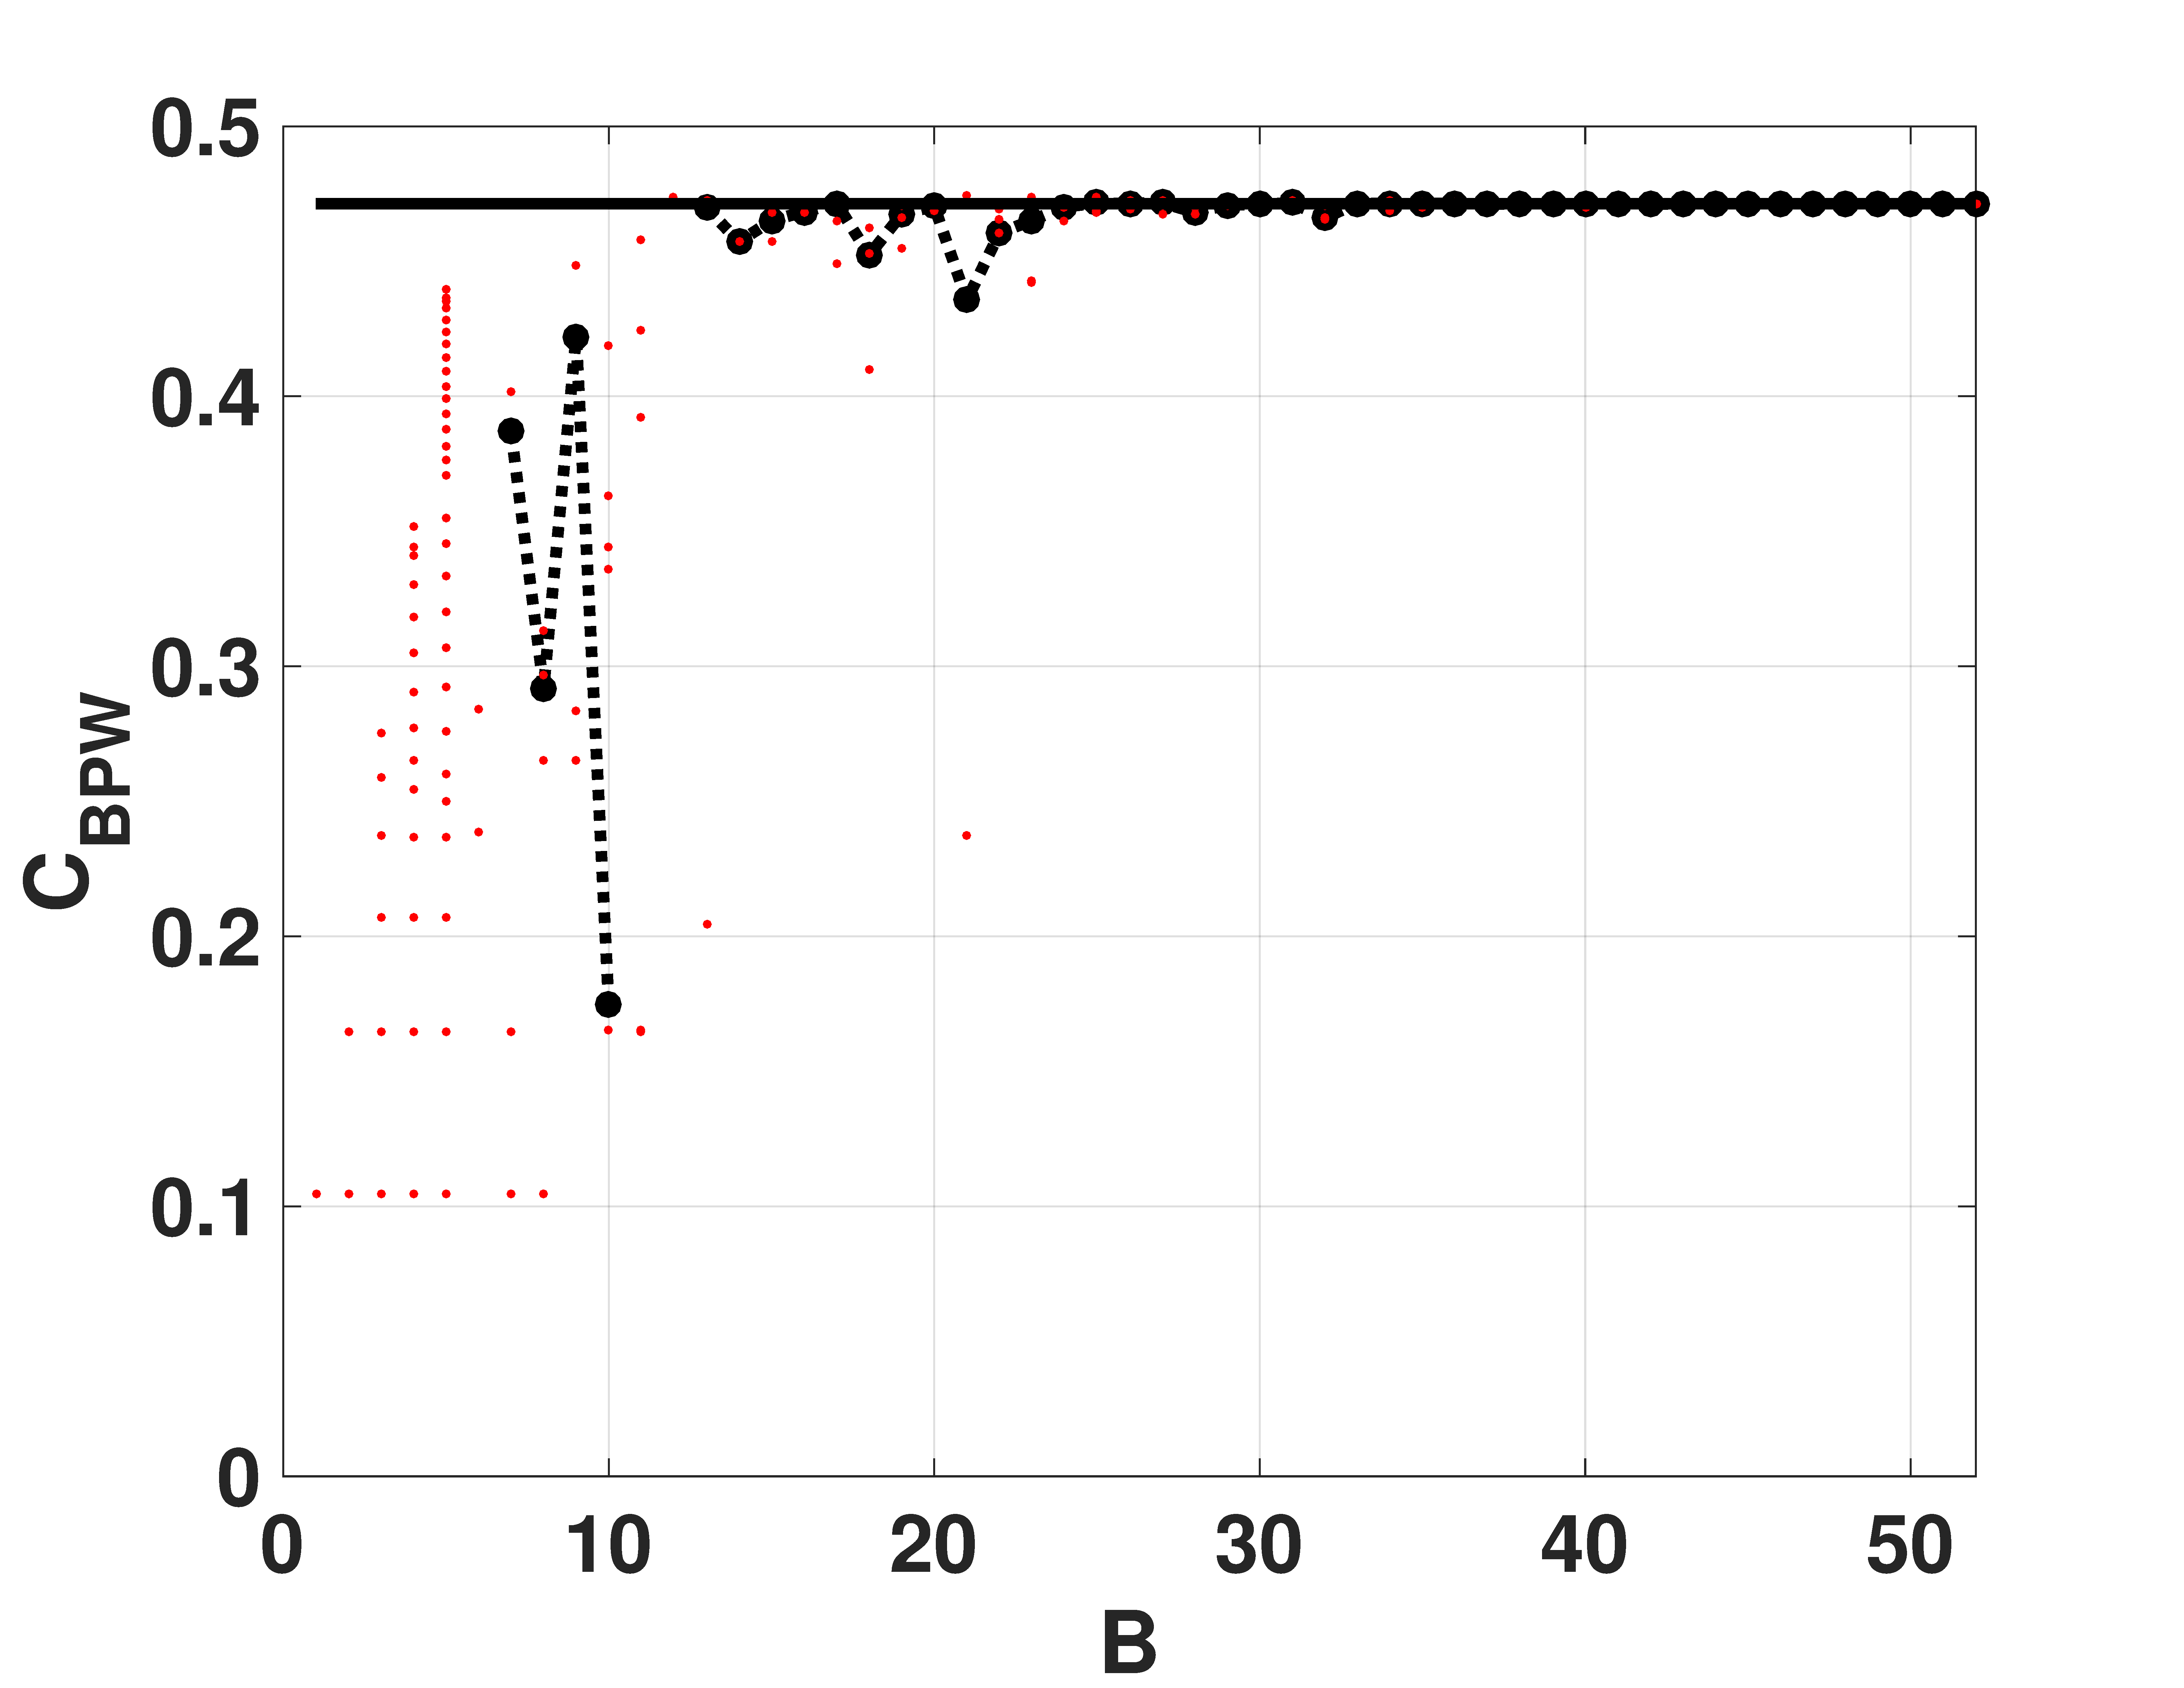
\includegraphics[width=\textwidth]{Cbpw_Tent1p96}
		\caption{$C_{BPW}$ vs. $B$}
		\label{fig:Cbpw_Tent1p96}
	\end{subfigure}
	\begin{subfigure}[b]{0.49\textwidth}
		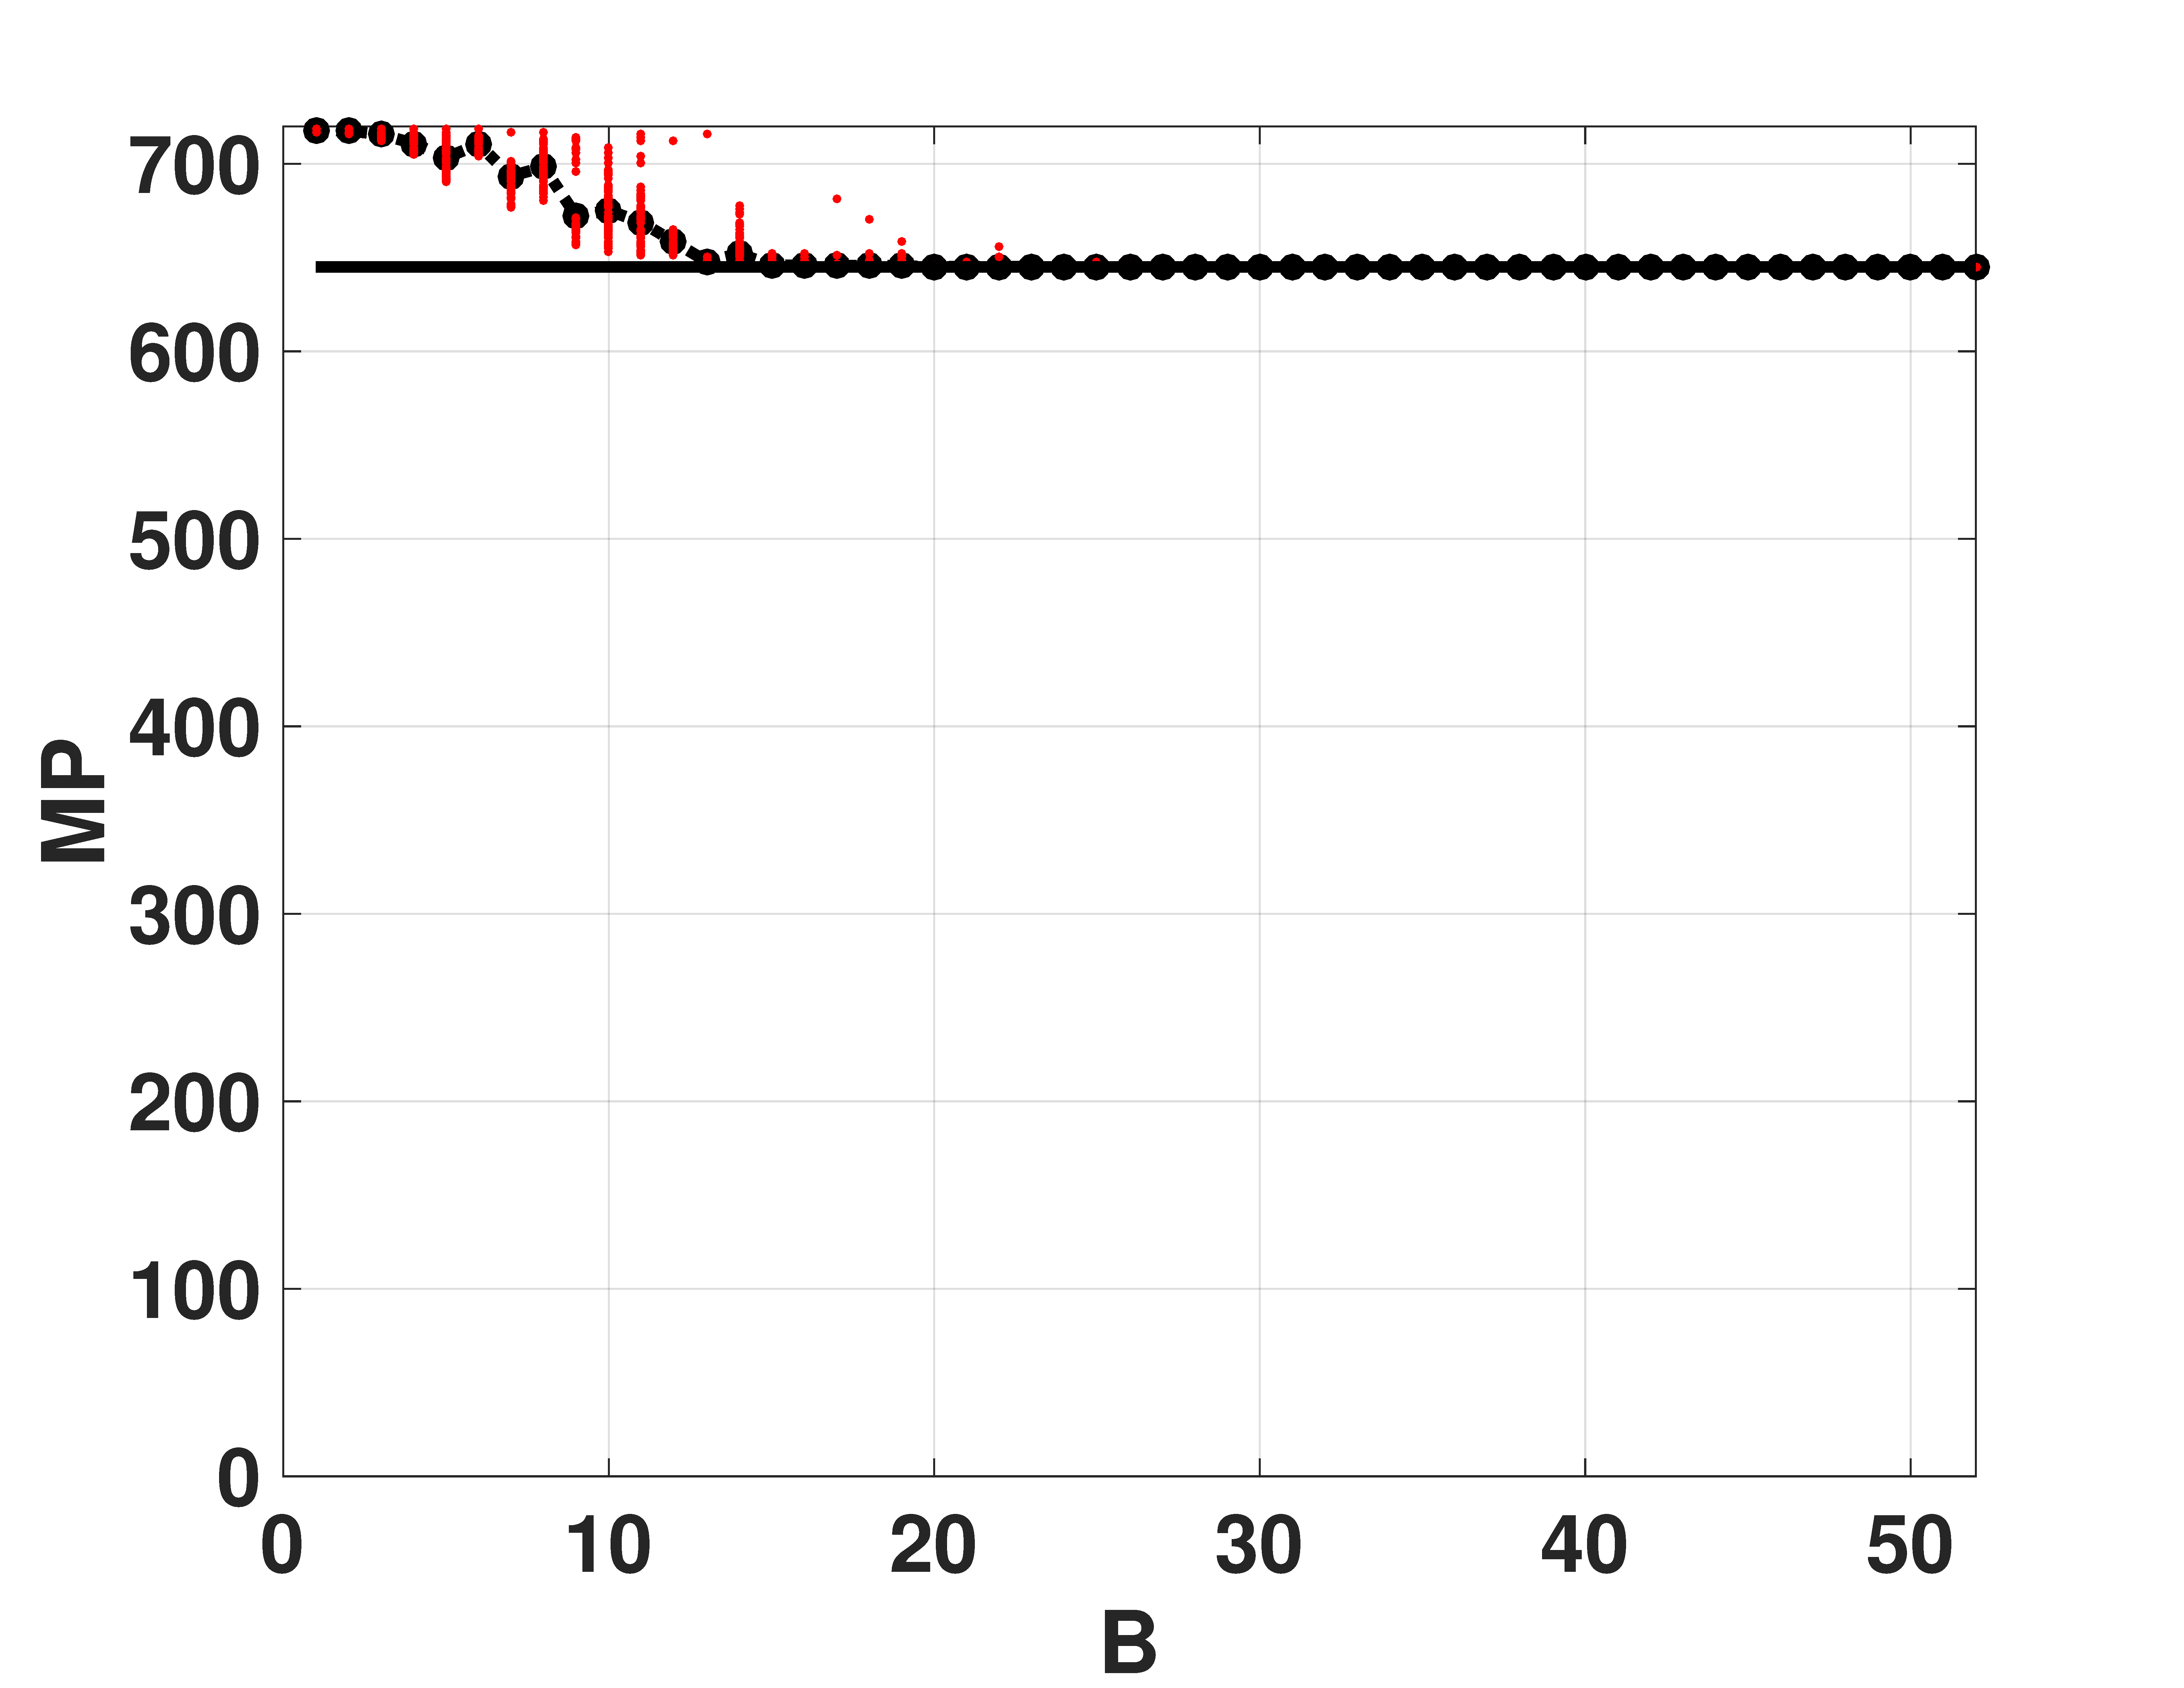
\includegraphics[width=\textwidth]{MP_Tent1p96}
		\caption{MP vs. $B$}
		\label{fig:MP_Tent1p96}
	\end{subfigure}
	\caption{Propiedades estadísticas del mapa TENT con $u=1.96$.}
	\label{fig:TENT1p96_QuantiB}
\end{figure}

Las posiciones en los planos doble entropía (Figura \ref{fig:TENT1p96_HH}) y entropía-complejidad (Figura \ref{fig:TENT1p96_HH}) son marginalmente mejores que los que se obtienen para el mapa LOG y son característicos de los mapas pseudocaóticos.
%
\begin{figure}[htpb]
	\centering
	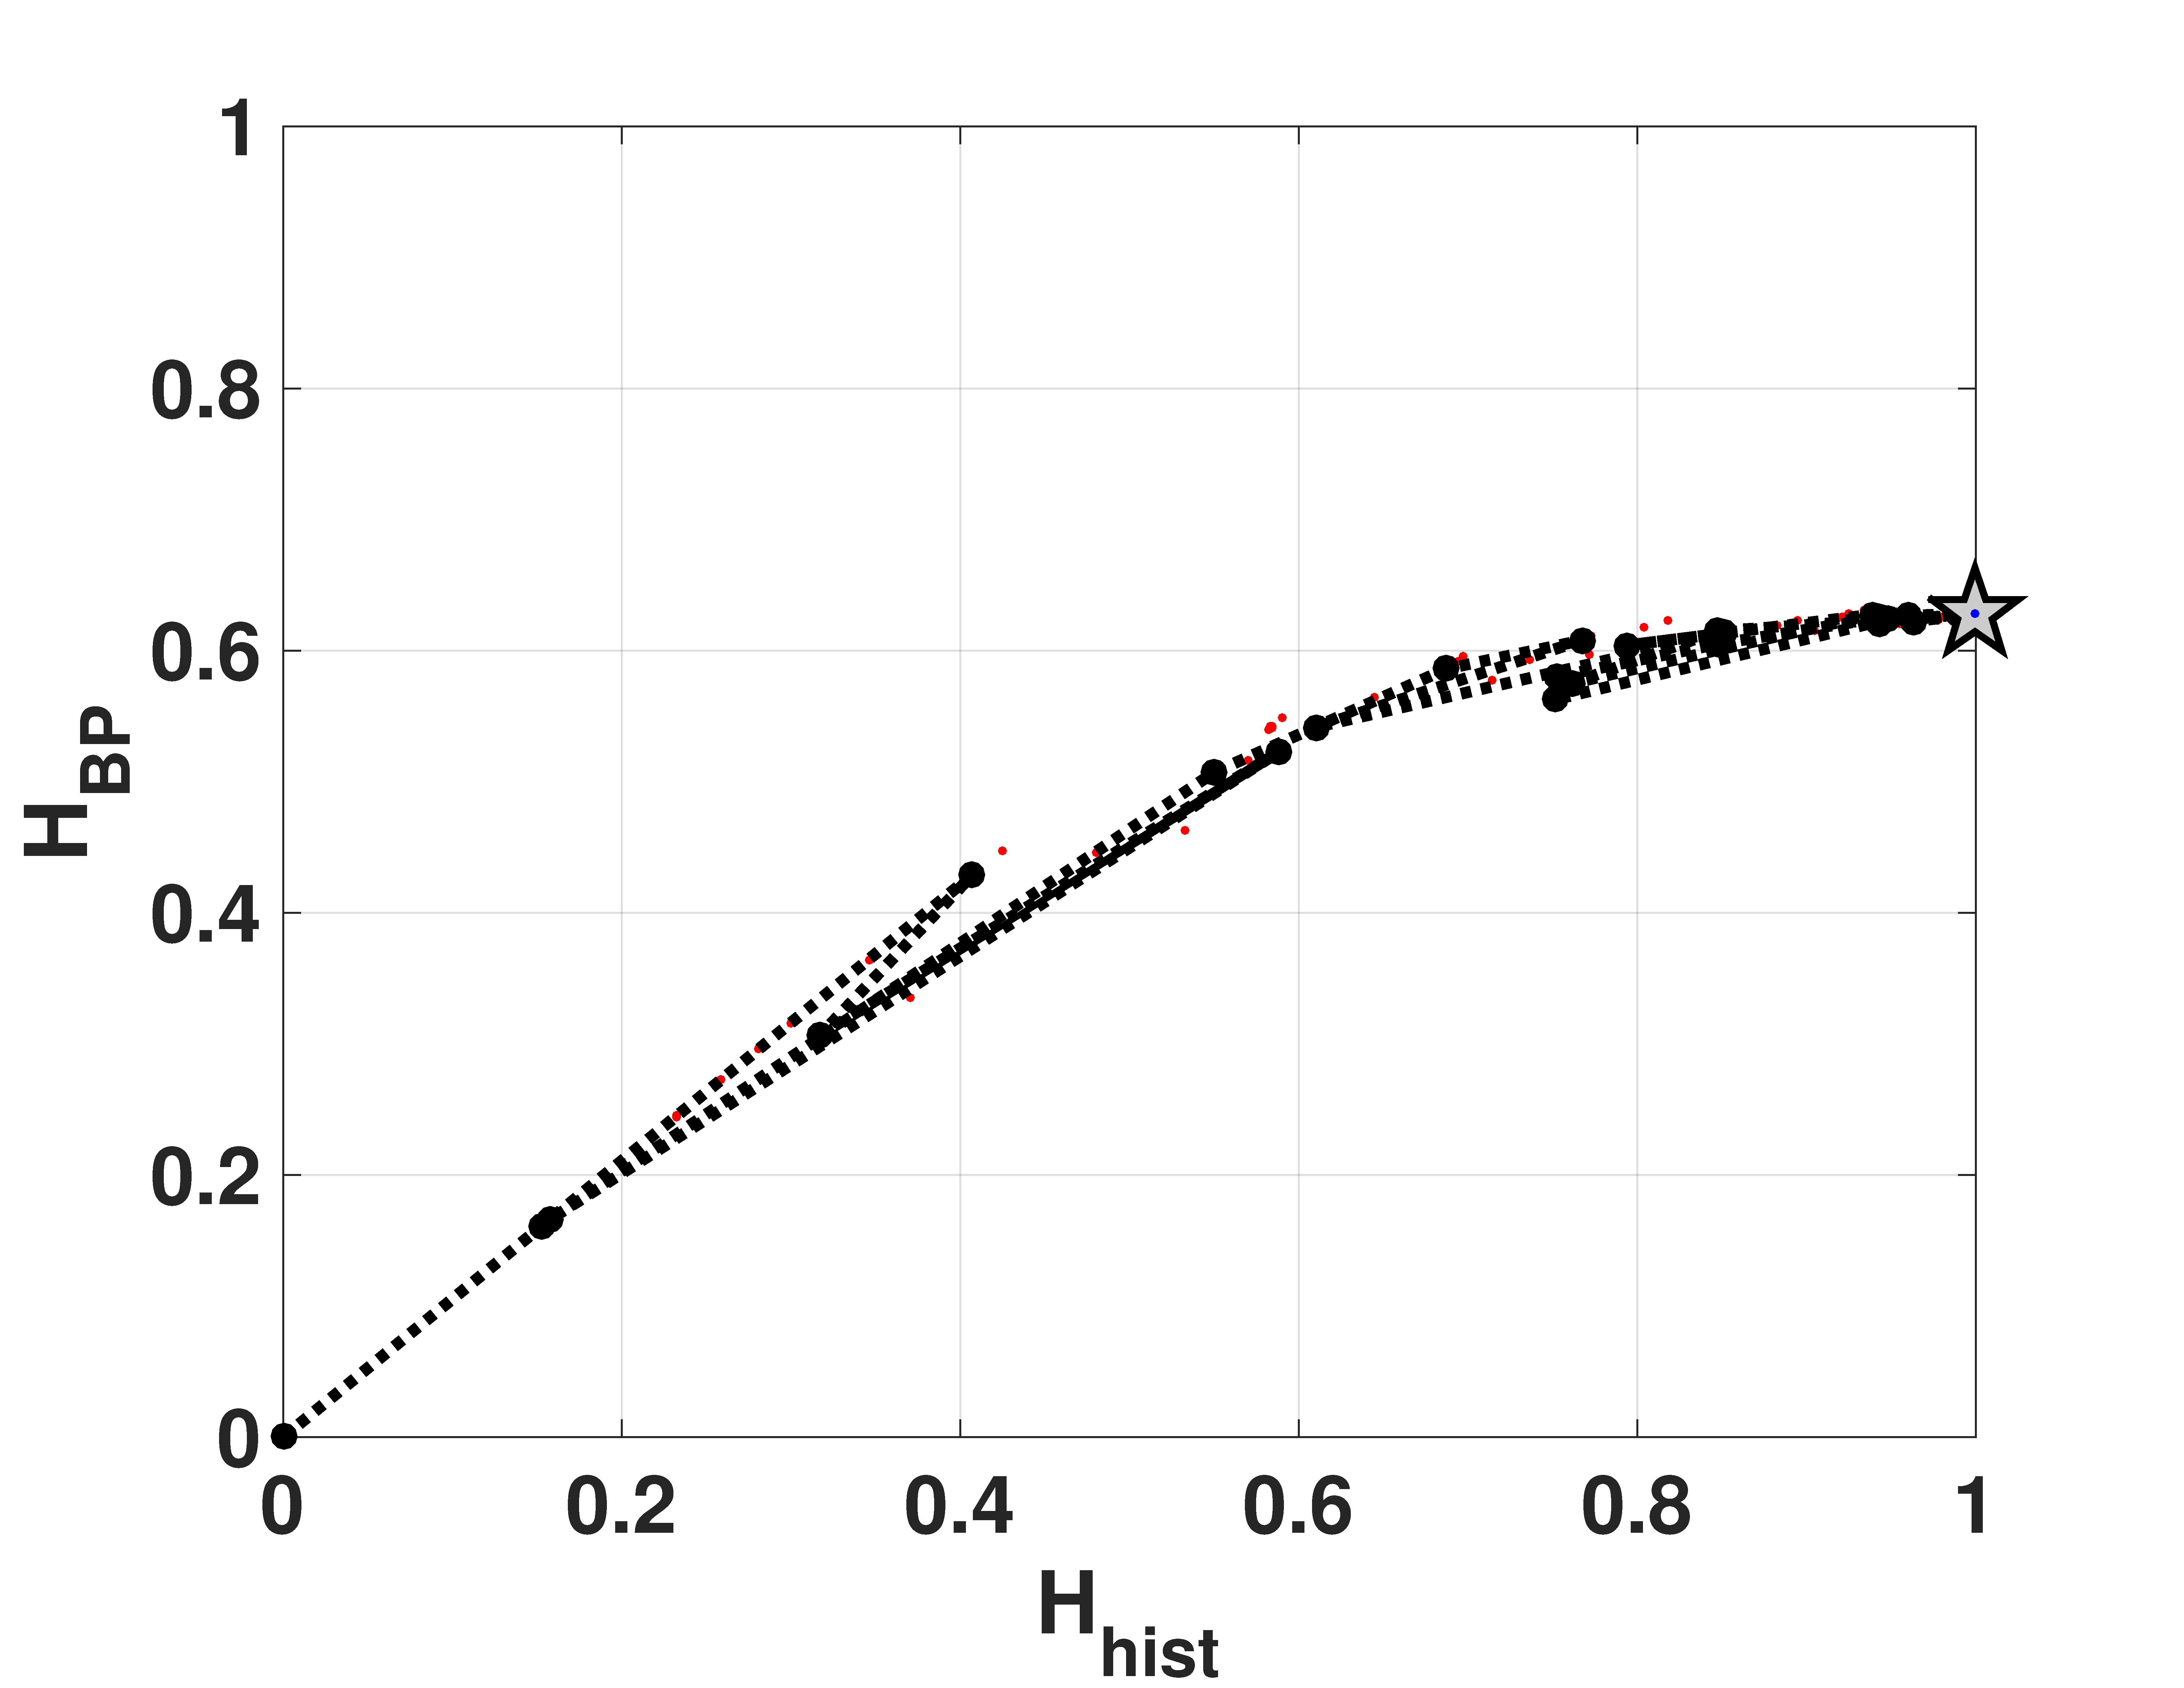
\includegraphics[width=.49\textwidth]{HbpHval_Tent1p96}
	\caption{Evolution of statistical properties in double entropy plane for TENT map with $u=1.96$.}
	\label{fig:TENT1p96_HH}
\end{figure}
%
\begin{figure}[htpb]
	\centering
	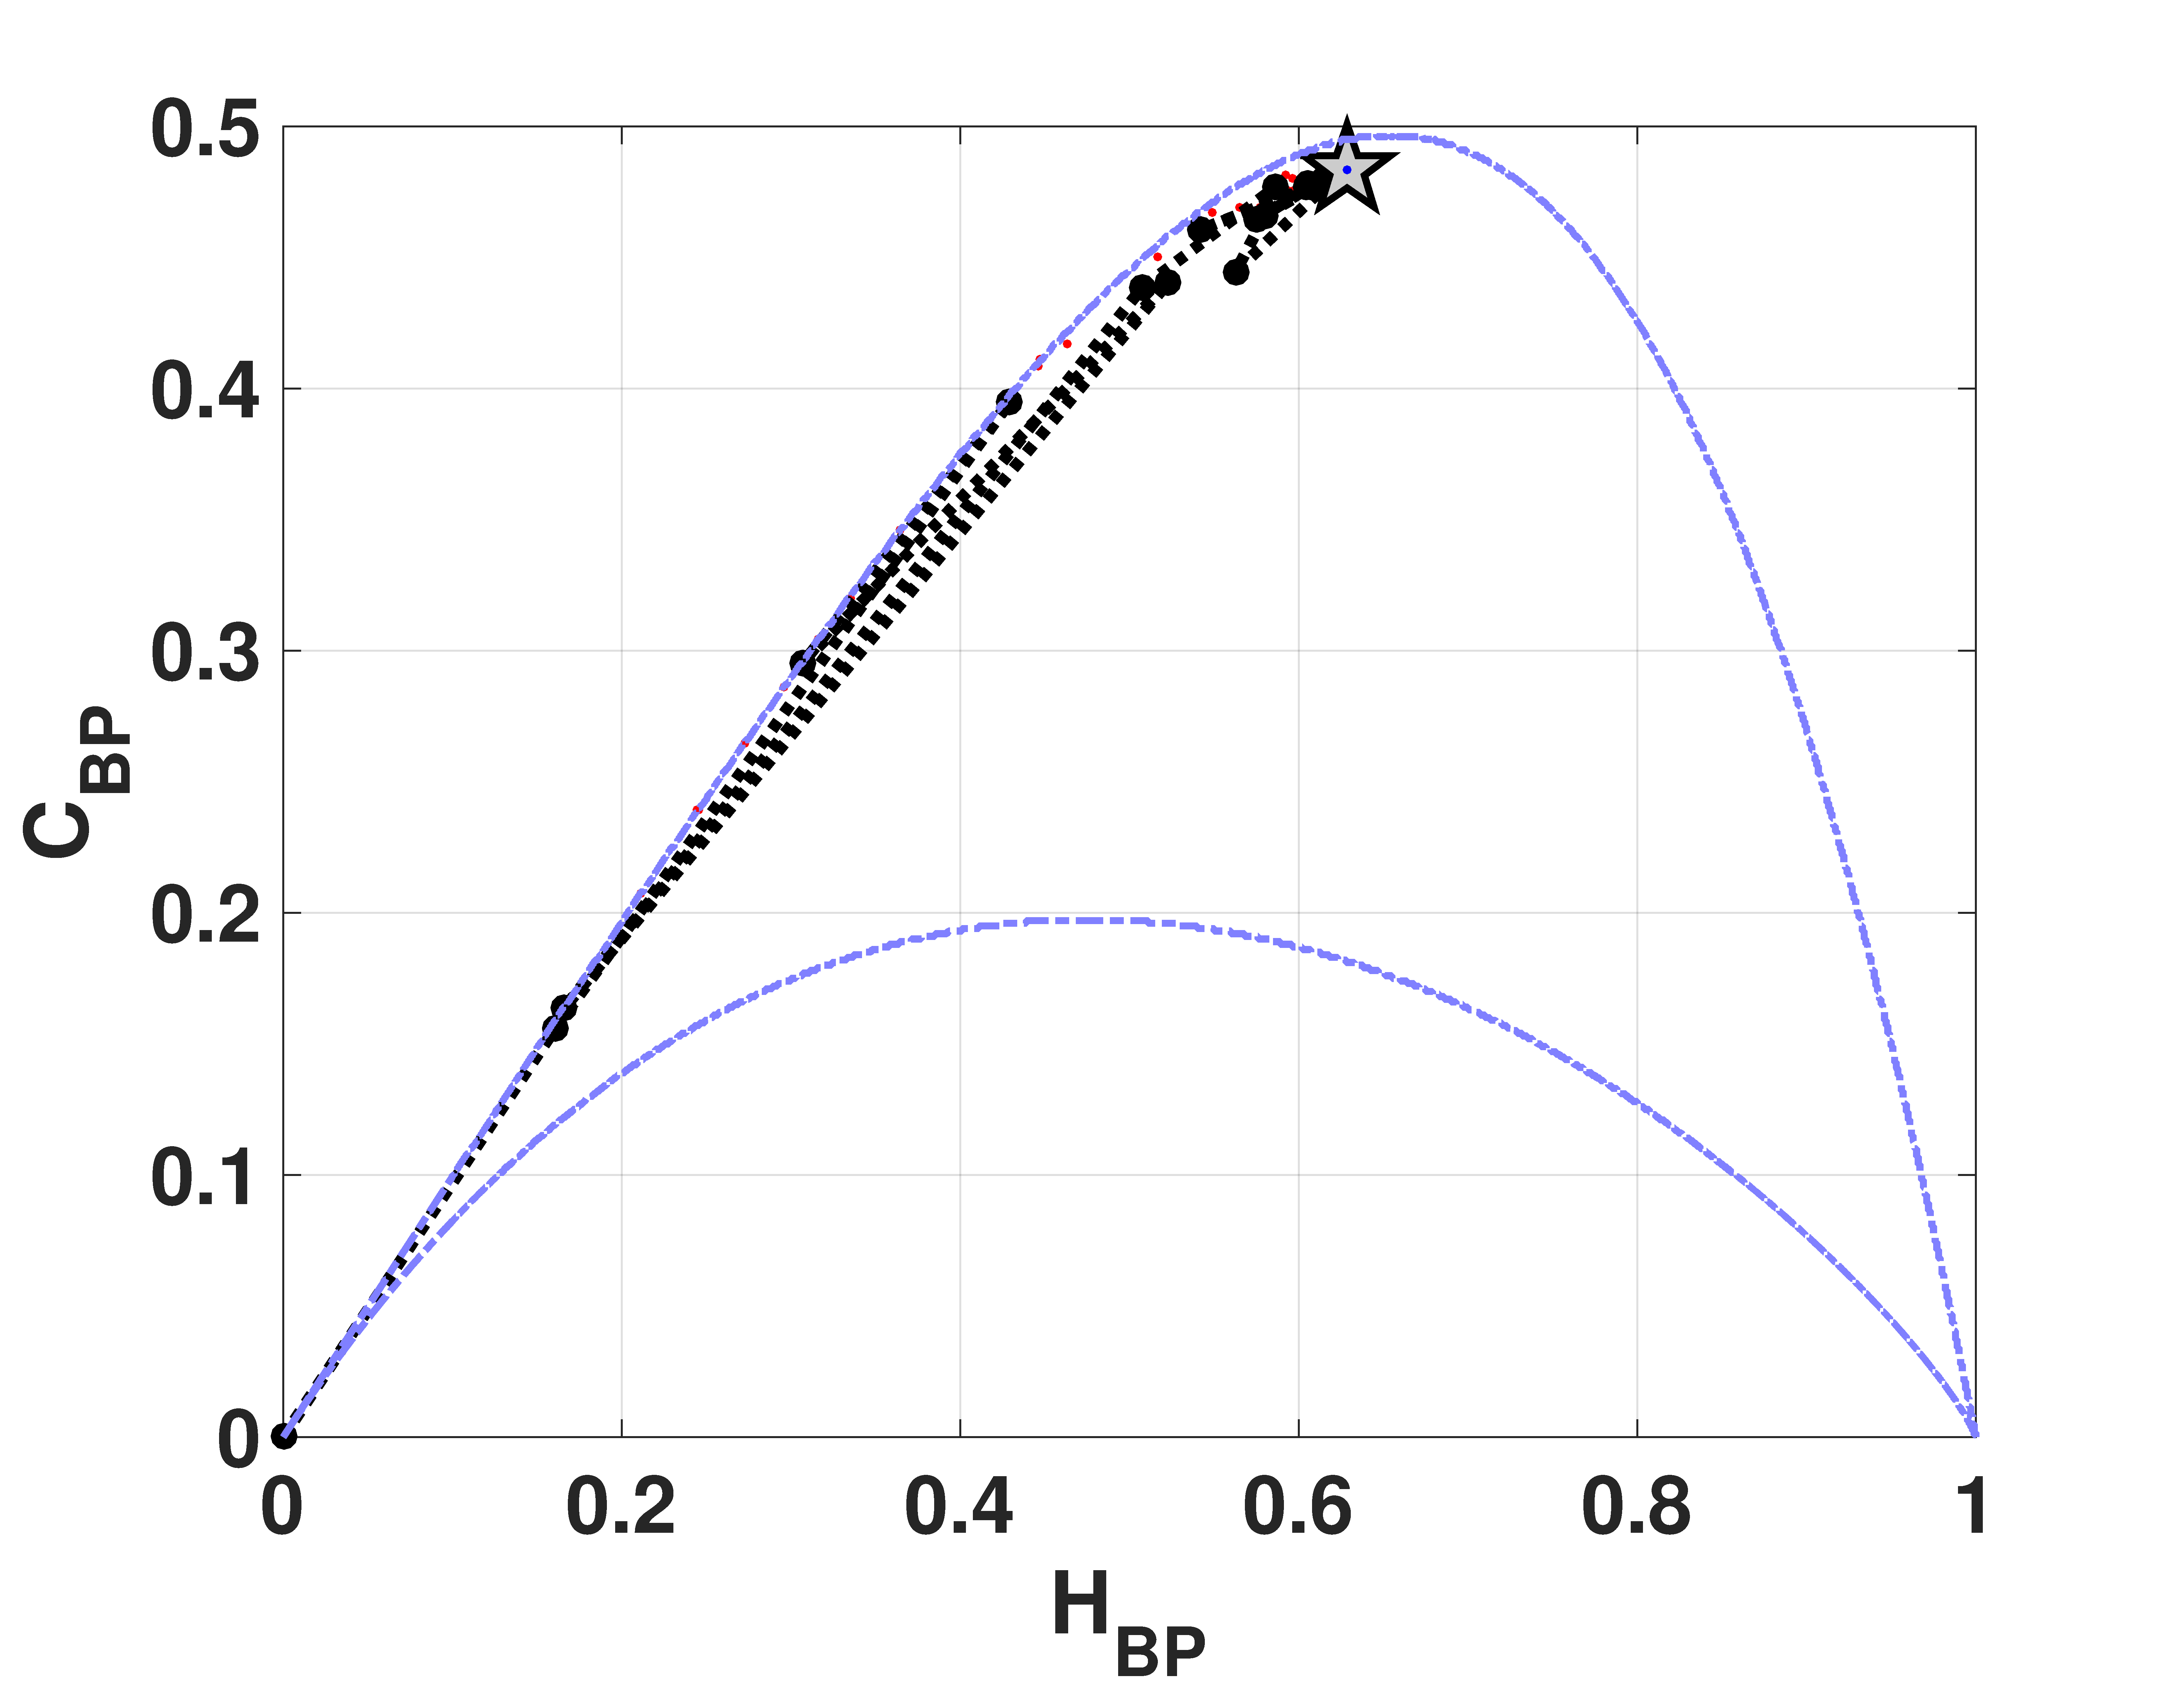
\includegraphics[width=.49\textwidth]{CbpHbp_Tent1p96}
	\caption{$H_{BP} \times C_{BP}$}
	\caption{Evolution of statistical properties in causal entropy-complexity plane for TENT map with $u=1.96$.}
	\label{fig:TENT1p96_HbpCbp}
\end{figure}